\chapter{范畴论基础}

\section{$2$-范畴}

\begin{definition}
	{($2$-范畴)}
	一个 $2$-范畴 $\mathcal C$ 包含如下资料:
	\begin{itemize}
		\item 
		\item
	\end{itemize}
	通常人们所说的 $2$-范畴是弱 $2$-范畴.
\end{definition}

\section{伴随函子}

谈论伴随的一个自然的语境是 $2$-范畴.

\begin{definition}
	{(伴随)}
	一个 $2$-范畴中的一组\emph{伴随}是
	\begin{itemize}
		\item 两个对象 $C,D$,
		\item 两个态射 $F\colon C\to D$, $G\colon D\to C$,
		\item 两个 $2$-态射 $\eta\colon \operatorname{id}_C\to GF$, $\varepsilon\colon FG\to\operatorname{id}_D$;
	\end{itemize}
	满足如下 $2$-态射的等式,
	\[\begin{tikzcd}[ampersand replacement=\&,column sep=1.5em]
		{C} \&\& {C} \\
		\& {D} \&\& {D}
		\arrow["F"', from=1-1, to=2-2]
		\arrow["G"{description}, from=2-2, to=1-3]
		\arrow["F", from=1-3, to=2-4]
		\arrow[""{name=0, anchor=center, inner sep=0}, "{\operatorname{id}_{\mathsf C}}", from=1-1, to=1-3]
		\arrow[""{name=1, anchor=center, inner sep=0}, "{\operatorname{id}_{\mathsf D}}"', from=2-2, to=2-4]
		\arrow["\eta"', shorten <=3pt, shorten >=3pt, Rightarrow, from=0, to=2-2]
		\arrow["\varepsilon", shorten <=3pt, shorten >=3pt, Rightarrow, from=1-3, to=1]
	\end{tikzcd}\hspace{-1em}=\operatorname{id}_F,
	\begin{tikzcd}[ampersand replacement=\&,column sep=1.5em]
		\& {C} \&\& {C} \\
		{D} \&\& {D}
		\arrow["G", from=2-1, to=1-2]
		\arrow["F"{description}, from=1-2, to=2-3]
		\arrow["G"', from=2-3, to=1-4]
		\arrow[""{name=0, anchor=center, inner sep=0}, "{\operatorname{id}_{\mathsf D}}"', from=2-1, to=2-3]
		\arrow[""{name=1, anchor=center, inner sep=0}, "{\operatorname{id}_{\mathsf C}}", from=1-2, to=1-4]
		\arrow["\varepsilon", shorten <=3pt, shorten >=3pt, Rightarrow, from=1-2, to=0]
		\arrow["\eta"', shorten <=3pt, shorten >=3pt, Rightarrow, from=1, to=2-3]
	\end{tikzcd}\hspace{-1em}=\operatorname{id}_{G}.\]

	这个条件也可用线图表示为

\tikzset{every picture/.style={line width=0.75pt}} %set default line width to 0.75pt        
\begin{center}
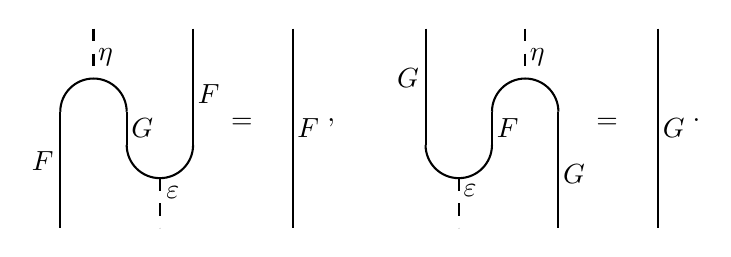
\begin{tikzpicture}[x=0.75pt,y=0.75pt,yscale=-0.8,xscale=0.8]
	%uncomment if require: \path (0,300); %set diagram left start at 0, and has height of 300
	
	%Straight Lines [id:da4698218774091225] 
	\draw    (100,130) -- (100,200) ;
	%Shape: Arc [id:dp5452146741155406] 
	\draw  [draw opacity=0] (100,130) .. controls (100,118.95) and (108.95,110) .. (120,110) .. controls (131.05,110) and (140,118.95) .. (140,130) -- (120,130) -- cycle ; \draw   (100,130) .. controls (100,118.95) and (108.95,110) .. (120,110) .. controls (131.05,110) and (140,118.95) .. (140,130) ;  
	%Shape: Arc [id:dp49645291516622003] 
	\draw  [draw opacity=0] (180,150) .. controls (180,150) and (180,150) .. (180,150) .. controls (180,150) and (180,150) .. (180,150) .. controls (180,161.05) and (171.05,170) .. (160,170) .. controls (148.95,170) and (140,161.05) .. (140,150) -- (160,150) -- cycle ; \draw   (180,150) .. controls (180,150) and (180,150) .. (180,150) .. controls (180,150) and (180,150) .. (180,150) .. controls (180,161.05) and (171.05,170) .. (160,170) .. controls (148.95,170) and (140,161.05) .. (140,150) ;  
	%Straight Lines [id:da07095399149030768] 
	\draw    (180,80) -- (180,150) ;
	%Straight Lines [id:da08445793804465951] 
	\draw  [dash pattern={on 4.5pt off 4.5pt}]  (120,80) -- (120,110) ;
	%Straight Lines [id:da40802862615686375] 
	\draw  [dash pattern={on 4.5pt off 4.5pt}]  (160,170) -- (160,200) ;
	%Straight Lines [id:da5905893191283564] 
	\draw    (140,130) -- (140,150) ;
	%Straight Lines [id:da7172863956237474] 
	\draw    (240,80) -- (240,200) ;
	%Straight Lines [id:da6534130406395566] 
	\draw    (320,80) -- (320,150) ;
	%Shape: Arc [id:dp37941315902148687] 
	\draw  [draw opacity=0] (360,130) .. controls (360,118.95) and (368.95,110) .. (380,110) .. controls (391.05,110) and (400,118.95) .. (400,130) -- (380,130) -- cycle ; \draw   (360,130) .. controls (360,118.95) and (368.95,110) .. (380,110) .. controls (391.05,110) and (400,118.95) .. (400,130) ;  
	%Shape: Arc [id:dp314690779386831] 
	\draw  [draw opacity=0] (360,150) .. controls (360,150) and (360,150) .. (360,150) .. controls (360,150) and (360,150) .. (360,150) .. controls (360,161.05) and (351.05,170) .. (340,170) .. controls (328.95,170) and (320,161.05) .. (320,150) -- (340,150) -- cycle ; \draw   (360,150) .. controls (360,150) and (360,150) .. (360,150) .. controls (360,150) and (360,150) .. (360,150) .. controls (360,161.05) and (351.05,170) .. (340,170) .. controls (328.95,170) and (320,161.05) .. (320,150) ;  
	%Straight Lines [id:da0821788481682626] 
	\draw    (400,130) -- (400,200) ;
	%Straight Lines [id:da026745112319709996] 
	\draw  [dash pattern={on 4.5pt off 4.5pt}]  (380,80) -- (380,110) ;
	%Straight Lines [id:da08383119415628326] 
	\draw  [dash pattern={on 4.5pt off 4.5pt}]  (340,170) -- (340,200) ;
	%Straight Lines [id:da867238855772305] 
	\draw    (360,130) -- (360,150) ;
	%Straight Lines [id:da7093402738130186] 
	\draw    (460,80) -- (460,200) ;
	
	% Text Node
	\draw (81,152) node [anchor=north west][inner sep=0.75pt]   [align=left] {$\displaystyle F$};
	% Text Node
	\draw (141,132) node [anchor=north west][inner sep=0.75pt]   [align=left] {$\displaystyle G$};
	% Text Node
	\draw (181,112) node [anchor=north west][inner sep=0.75pt]   [align=left] {$\displaystyle F$};
	% Text Node
	\draw (201,132) node [anchor=north west][inner sep=0.75pt]   [align=left] {$\displaystyle =$};
	% Text Node
	\draw (241,132) node [anchor=north west][inner sep=0.75pt]   [align=left] {$\displaystyle F$};
	% Text Node
	\draw (301,102) node [anchor=north west][inner sep=0.75pt]   [align=left] {$\displaystyle G$};
	% Text Node
	\draw (361,132) node [anchor=north west][inner sep=0.75pt]   [align=left] {$\displaystyle F$};
	% Text Node
	\draw (421,132) node [anchor=north west][inner sep=0.75pt]   [align=left] {$\displaystyle =$};
	% Text Node
	\draw (461,132) node [anchor=north west][inner sep=0.75pt]   [align=left] {$\displaystyle G$};
	% Text Node
	\draw (401,160) node [anchor=north west][inner sep=0.75pt]   [align=left] {$\displaystyle G$};
	% Text Node
	\draw (259,132) node [anchor=north west][inner sep=0.75pt]   [align=left] {$\displaystyle ,$};
	% Text Node
	\draw (479,132) node [anchor=north west][inner sep=0.75pt]   [align=left] {$\displaystyle .$};
	% Text Node
	\draw (121,90) node [anchor=north west][inner sep=0.75pt]   [align=left] {$\displaystyle \eta $};
	% Text Node
	\draw (162,173) node [anchor=north west][inner sep=0.75pt]   [align=left] {$\displaystyle \varepsilon $};
	% Text Node
	\draw (341,172) node [anchor=north west][inner sep=0.75pt]   [align=left] {$\displaystyle \varepsilon $};
	% Text Node
	\draw (381,90) node [anchor=north west][inner sep=0.75pt]   [align=left] {$\displaystyle \eta $};
	
	
\end{tikzpicture}
\end{center}

\end{definition}

\begin{example}
	{(伴随函子)}
	$2$-范畴 $\mathsf {Cat}$ 中的伴随就是熟知的伴随函子. 对于伴随函子 $F\colon \mathsf C\to\mathsf D$, $G\colon \mathsf D\to\mathsf C$, 如下的线图给出了映射
	$$
	\operatorname{Hom}(Fc,d) \to \operatorname{Hom}(c,Gd).
	$$
	\begin{center}
		
		
		\tikzset{every picture/.style={line width=0.75pt}} %set default line width to 0.75pt        
		
		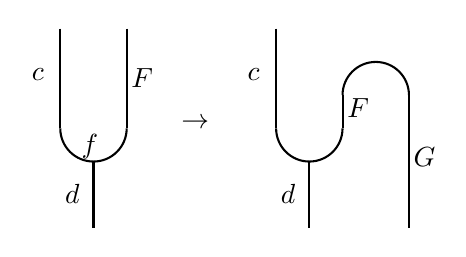
\begin{tikzpicture}[x=0.75pt,y=0.75pt,yscale=-0.8,xscale=0.8]
			%uncomment if require: \path (0,300); %set diagram left start at 0, and has height of 300
			
			%Straight Lines [id:da38389280296337147] 
			\draw    (70,100) -- (70,160) ;
			%Shape: Arc [id:dp500451274224406] 
			\draw  [draw opacity=0] (110,160) .. controls (110,160) and (110,160) .. (110,160) .. controls (110,160) and (110,160) .. (110,160) .. controls (110,171.05) and (101.05,180) .. (90,180) .. controls (78.95,180) and (70,171.05) .. (70,160) -- (90,160) -- cycle ; \draw   (110,160) .. controls (110,160) and (110,160) .. (110,160) .. controls (110,160) and (110,160) .. (110,160) .. controls (110,171.05) and (101.05,180) .. (90,180) .. controls (78.95,180) and (70,171.05) .. (70,160) ;  
			%Straight Lines [id:da36761146974596803] 
			\draw    (110,100) -- (110,160) ;
			%Straight Lines [id:da28528438514767007] 
			\draw    (90,180) -- (90,220) ;
			%Straight Lines [id:da2956003592318719] 
			\draw    (200,100) -- (200,160) ;
			%Shape: Arc [id:dp007579126105482503] 
			\draw  [draw opacity=0] (240,160) .. controls (240,160) and (240,160) .. (240,160) .. controls (240,160) and (240,160) .. (240,160) .. controls (240,171.05) and (231.05,180) .. (220,180) .. controls (208.95,180) and (200,171.05) .. (200,160) -- (220,160) -- cycle ; \draw   (240,160) .. controls (240,160) and (240,160) .. (240,160) .. controls (240,160) and (240,160) .. (240,160) .. controls (240,171.05) and (231.05,180) .. (220,180) .. controls (208.95,180) and (200,171.05) .. (200,160) ;  
			%Straight Lines [id:da48802759810410334] 
			\draw    (240,140) -- (240,160) ;
			%Straight Lines [id:da20597425552353443] 
			\draw    (220,180) -- (220,220) ;
			%Shape: Arc [id:dp2471225279229352] 
			\draw  [draw opacity=0] (240,140) .. controls (240,128.95) and (248.95,120) .. (260,120) .. controls (271.05,120) and (280,128.95) .. (280,140) -- (260,140) -- cycle ; \draw   (240,140) .. controls (240,128.95) and (248.95,120) .. (260,120) .. controls (271.05,120) and (280,128.95) .. (280,140) ;  
			%Straight Lines [id:da42525487208205326] 
			\draw    (280,140) -- (280,220) ;
			
			% Text Node
			\draw (141,152) node [anchor=north west][inner sep=0.75pt]   [align=left] {$\displaystyle \rightarrow $};
			% Text Node
			\draw (51,122) node [anchor=north west][inner sep=0.75pt]   [align=left] {$\displaystyle c$};
			% Text Node
			\draw (111,122) node [anchor=north west][inner sep=0.75pt]   [align=left] {$\displaystyle F$};
			% Text Node
			\draw (71,192) node [anchor=north west][inner sep=0.75pt]   [align=left] {$\displaystyle d$};
			% Text Node
			\draw (81,162) node [anchor=north west][inner sep=0.75pt]   [align=left] {$\displaystyle f$};
			% Text Node
			\draw (181,122) node [anchor=north west][inner sep=0.75pt]   [align=left] {$\displaystyle c$};
			% Text Node
			\draw (241,140) node [anchor=north west][inner sep=0.75pt]   [align=left] {$\displaystyle F$};
			% Text Node
			\draw (281,170) node [anchor=north west][inner sep=0.75pt]   [align=left] {$\displaystyle G$};
			% Text Node
			\draw (201,192) node [anchor=north west][inner sep=0.75pt]   [align=left] {$\displaystyle d$};
			
			
		\end{tikzpicture}
	\end{center}
	其中我们将对象 $c$ 视为函子 $1\to\mathsf C$. 考虑一个形如
	\tikzset{every picture/.style={line width=0.75pt}} %set default line width to 0.75pt        
	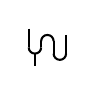
\begin{tikzpicture}[x=0.75pt,y=0.75pt,yscale=-0.15,xscale=0.15]
		%uncomment if require: \path (0,300); %set diagram left start at 0, and has height of 300
		
		%Straight Lines [id:da9426120658362054] 
		\draw    (200,100) -- (200,160) ;
		%Shape: Arc [id:dp7574128344072426] 
		\draw  [draw opacity=0] (240,160) .. controls (240,160) and (240,160) .. (240,160) .. controls (240,160) and (240,160) .. (240,160) .. controls (240,171.05) and (231.05,180) .. (220,180) .. controls (208.95,180) and (200,171.05) .. (200,160) -- (220,160) -- cycle ; \draw   (240,160) .. controls (240,160) and (240,160) .. (240,160) .. controls (240,160) and (240,160) .. (240,160) .. controls (240,171.05) and (231.05,180) .. (220,180) .. controls (208.95,180) and (200,171.05) .. (200,160) ;  
		%Straight Lines [id:da6440236067654423] 
		\draw    (240,140) -- (240,160) ;
		%Straight Lines [id:da6278109278126796] 
		\draw    (220,180) -- (220,220) ;
		%Shape: Arc [id:dp5036962649695886] 
		\draw  [draw opacity=0] (240,140) .. controls (240,128.95) and (248.95,120) .. (260,120) .. controls (271.05,120) and (280,128.95) .. (280,140) -- (260,140) -- cycle ; \draw   (240,140) .. controls (240,128.95) and (248.95,120) .. (260,120) .. controls (271.05,120) and (280,128.95) .. (280,140) ;  
		%Straight Lines [id:da8724403377021124] 
		\draw    (280,140) -- (280,180) ;
		%Shape: Arc [id:dp2997750340889149] 
		\draw  [draw opacity=0] (320,180) .. controls (320,180) and (320,180) .. (320,180) .. controls (320,180) and (320,180) .. (320,180) .. controls (320,191.05) and (311.05,200) .. (300,200) .. controls (288.95,200) and (280,191.05) .. (280,180) -- (300,180) -- cycle ; \draw   (320,180) .. controls (320,180) and (320,180) .. (320,180) .. controls (320,180) and (320,180) .. (320,180) .. controls (320,191.05) and (311.05,200) .. (300,200) .. controls (288.95,200) and (280,191.05) .. (280,180) ;  
		%Straight Lines [id:da9641461547001391] 
		\draw    (320,120) -- (320,180) ;
	\end{tikzpicture}
	的线图, 我们得到上述映射为同构.
\end{example}

\subsection{伴随保持极限}

\begin{prop}
	[label={adjoints-preserve-limits}]
	{}
	右伴随保持极限, 左伴随保持余极限.
\end{prop}

\begin{proof}
	设有伴随
	% https://q.uiver.app/#q=WzAsMixbMCwwLCJcXG1hdGhzZiB7Q30iXSxbMSwwLCJcXG1hdGhzZiB7RH0iXSxbMSwwLCJGIiwyLHsib2Zmc2V0IjoyfV0sWzAsMSwiRyIsMix7Im9mZnNldCI6Mn1dLFsyLDMsIiIsMCx7ImxldmVsIjoxLCJzdHlsZSI6eyJuYW1lIjoiYWRqdW5jdGlvbiJ9fV1d
	\[\begin{tikzcd}[ampersand replacement=\&]
		{\mathsf {C}} \& {\mathsf {D},}
		\arrow[""{name=0, anchor=center, inner sep=0}, "F"', shift right=2, from=1-2, to=1-1]
		\arrow[""{name=1, anchor=center, inner sep=0}, "G"', shift right=2, from=1-1, to=1-2]
		\arrow["\dashv"{anchor=center, rotate=-90}, draw=none, from=0, to=1]
	\end{tikzcd}\]
	设 $X \colon I \to \mathsf C$ 是一个图 ($I$ 是小范畴).
	若极限 $\lim_i X_i$ 存在,
	则有自然同构
	\begin{align*}
		\operatorname{Hom}(-,G\lim_i X_i)
		&\simeq \operatorname{Hom}(F-,\lim_i X_i)\\
		&\simeq \lim_i \operatorname{Hom}(F-,X_i)\\
		&\simeq \lim_i \operatorname{Hom}(-,GX_i)\\
		&\simeq \operatorname{Hom}(-,\lim_i GX_i).
	\end{align*}
	由米田引理, 得同构 $G\lim_i X_i \simeq \lim_i GX_i$,
	故右伴随保持极限.
	另一结论由对偶性即证.
\end{proof}

\begin{example}
	[label={Top-Set-adjunction}]
	{}
	遗忘函子 $\mathsf {Top} \to \mathsf {Set}$ 同时有左伴随和右伴随.
	% https://q.uiver.app/#q=WzAsMixbMCwwLCJcXG1hdGhzZiB7VG9wfSJdLFsyLDAsIlxcbWF0aHNmIHtTZXR9Il0sWzAsMSwiXFx0ZXh0e+mBl+W/mH0iLDAseyJsYWJlbF9wb3NpdGlvbiI6MjB9XSxbMSwwLCLnprvmlaMiLDIseyJsYWJlbF9wb3NpdGlvbiI6MjAsIm9mZnNldCI6NX1dLFsxLDAsIuW5s+WHoSIsMCx7ImxhYmVsX3Bvc2l0aW9uIjoyMCwib2Zmc2V0IjotNX1dLFszLDIsIiIsMSx7ImxldmVsIjoxLCJzdHlsZSI6eyJuYW1lIjoiYWRqdW5jdGlvbiJ9fV0sWzIsNCwiIiwxLHsibGV2ZWwiOjEsInN0eWxlIjp7Im5hbWUiOiJhZGp1bmN0aW9uIn19XV0=
	\[\begin{tikzcd}[ampersand replacement=\&]
		{\mathsf {Top}} \&\& {\mathsf {Set}}
		\arrow[""{name=0, anchor=center, inner sep=0}, "{\text{遗忘}}"{pos=0.2}, from=1-1, to=1-3]
		\arrow[""{name=1, anchor=center, inner sep=0}, "{\text{离散}}"'{pos=0.2}, shift right=5, from=1-3, to=1-1]
		\arrow[""{name=2, anchor=center, inner sep=0}, "{\text{平凡}}"{pos=0.2}, shift left=5, from=1-3, to=1-1]
		\arrow["\dashv"{anchor=center, rotate=-90}, draw=none, from=1, to=0]
		\arrow["\dashv"{anchor=center, rotate=-90}, draw=none, from=0, to=2]
	\end{tikzcd}\]
	因此这个遗忘同时保持极限与余极限; 换言之, 拓扑空间的极限与余极限可用底层集合的极限与余极限来计算.
\end{example}


\begin{example}
	[label={Gpd-Cat-adjunction}]
	{}
	群胚是一种特殊的范畴, 即有嵌入 $i\colon \mathsf {Gpd} \to \mathsf {Cat}$. 这个函子同时有左伴随和右伴随.
	% https://q.uiver.app/#q=WzAsMixbMCwwLCJcXG1hdGhzZiB7VG9wfSJdLFsyLDAsIlxcbWF0aHNmIHtTZXR9Il0sWzAsMSwiXFx0ZXh0e+mBl+W/mH0iLDAseyJsYWJlbF9wb3NpdGlvbiI6MjB9XSxbMSwwLCLnprvmlaMiLDIseyJsYWJlbF9wb3NpdGlvbiI6MjAsIm9mZnNldCI6NX1dLFsxLDAsIuW5s+WHoSIsMCx7ImxhYmVsX3Bvc2l0aW9uIjoyMCwib2Zmc2V0IjotNX1dLFszLDIsIiIsMSx7ImxldmVsIjoxLCJzdHlsZSI6eyJuYW1lIjoiYWRqdW5jdGlvbiJ9fV0sWzIsNCwiIiwxLHsibGV2ZWwiOjEsInN0eWxlIjp7Im5hbWUiOiJhZGp1bmN0aW9uIn19XV0=
	\[\begin{tikzcd}[ampersand replacement=\&]
		{\mathsf {Gpd}} \&\& {\mathsf {Cat}}
		\arrow[""{name=0, anchor=center, inner sep=0}, "{i}"{pos=0.2}, from=1-1, to=1-3]
		\arrow[""{name=1, anchor=center, inner sep=0}, "{\pi_1}"'{pos=0.2}, shift right=5, from=1-3, to=1-1]
		\arrow[""{name=2, anchor=center, inner sep=0}, "{\text{极大子群胚}}"{pos=0.35}, shift left=5, from=1-3, to=1-1]
		\arrow["\dashv"{anchor=center, rotate=-90}, draw=none, from=1, to=0]
		\arrow["\dashv"{anchor=center, rotate=-90}, draw=none, from=0, to=2]
	\end{tikzcd}\]
	(其中 $\pi_1$ 给出范畴的基本群胚, 即一个范畴中 ``形式地加入所有态射的逆'' 得到的群胚.)
	因此 $i$ 同时保持极限与余极限.
\end{example}

\begin{prop}
	[label={adjoint-full-subcategory-equivalence}]
	{(伴随产生一对满子范畴的等价)}
	设有伴随
	% https://q.uiver.app/#q=WzAsMixbMCwwLCJcXG1hdGhzZiB7Q30iXSxbMSwwLCJcXG1hdGhzZiB7RH0iXSxbMSwwLCJGIiwyLHsib2Zmc2V0IjoyfV0sWzAsMSwiRyIsMix7Im9mZnNldCI6Mn1dLFsyLDMsIiIsMCx7ImxldmVsIjoxLCJzdHlsZSI6eyJuYW1lIjoiYWRqdW5jdGlvbiJ9fV1d
	\[\begin{tikzcd}[ampersand replacement=\&]
		{\mathsf {C}} \& {\mathsf {D},}
		\arrow[""{name=0, anchor=center, inner sep=0}, "F"', shift right=2, from=1-2, to=1-1]
		\arrow[""{name=1, anchor=center, inner sep=0}, "G"', shift right=2, from=1-1, to=1-2]
		\arrow["\dashv"{anchor=center, rotate=-90}, draw=none, from=0, to=1]
	\end{tikzcd}\]
	其单位和余单位分别为
	$\eta \colon \operatorname{id}_{\mathsf D} \to GF$,
	$\epsilon \colon FG \to \operatorname{id}_{\mathsf C}$.
	考虑
	\begin{itemize}
		\item $\mathsf C$ 中由使得 $\eta_X \colon X \to GF(X)$ 为同构的 $X$ 构成的满子范畴 $\widetilde {\mathsf C}$,
		以及
		\item $\mathsf D$ 中由使得 $\epsilon_Y \colon FG(Y)\to Y$ 为同构的 $Y$ 构成的满子范畴 $\widetilde {\mathsf D}$,
	\end{itemize}
	那么 $F$ 与 $G$ 限制为一对互逆的范畴等价
	$$
	\widetilde G\colon \widetilde {\mathsf C} \overset{\simeq}{\to} \widetilde {\mathsf D},\quad
	\widetilde F\colon \widetilde {\mathsf D} \overset{\simeq}{\to} \widetilde {\mathsf C}.
	$$
\end{prop}

\begin{proof}
	由条件, $\eta$ 限制为自然变换
	$$
	\widetilde \eta \colon
	\operatorname{id}_{\widetilde {\mathsf D}} \to \widetilde G \widetilde F,
	$$
	且 $\widetilde \eta$ 的每个分量 ${\widetilde \eta}_{X} \colon X \to \widetilde G \widetilde F (X)$ 均为同构.
	因此 $\widetilde \eta$ 为自然同构. 另一边类似.
\end{proof}

\subsection{伴随三元组}

\begin{definition}
	{(伴随三元组)}
	范畴 (或一般 $2$-范畴中的对象) $\mathsf {C},\mathsf {D}$ 之间的\emph{伴随三元组} (adjoint triple) 是如下三个函子与两组伴随,
	\[\begin{tikzcd}[ampersand replacement=\&,column sep=2em]
		{\mathsf {C}} \&\& {\mathsf {D}.}
		\arrow[""{name=0, anchor=center, inner sep=0}, "{G}"{pos=0.2}, from=1-1, to=1-3]
		\arrow[""{name=1, anchor=center, inner sep=0}, "{F}"'{pos=0.2}, shift right=5, from=1-3, to=1-1]
		\arrow[""{name=2, anchor=center, inner sep=0}, "{H}"{pos=0.35}, shift left=5, from=1-3, to=1-1]
		\arrow["\dashv"{anchor=center, rotate=-90}, draw=none, from=1, to=0]
		\arrow["\dashv"{anchor=center, rotate=-90}, draw=none, from=0, to=2]
	\end{tikzcd}\]
\end{definition}

\begin{prop}
	{(伴随三元组诱导伴随)}
	伴随三元组 $F\dashv G \dashv H$ 诱导两对伴随
	$
	GF\dashv GH,
	FG\dashv HG.
	$
\end{prop}
\begin{proof}
	对于伴随函子, 结论很容易验证. 对一般的 $2$-范畴中的伴随, 其证明 (的一部分) 可用线图表示如下.
	\vspace{-1em}\begin{center}
		\tikzset{every picture/.style={line width=0.75pt}} %set default line width to 0.75pt        
		
		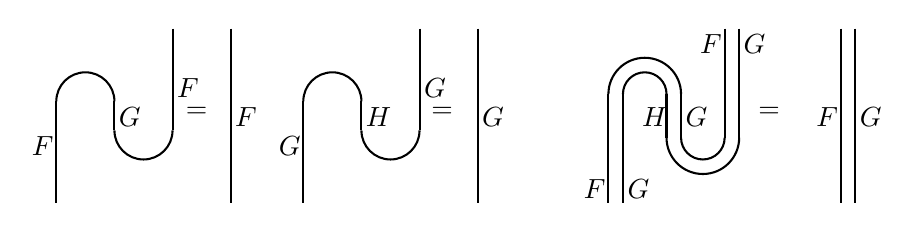
\begin{tikzpicture}[x=0.75pt,y=0.75pt,yscale=-0.7,xscale=0.7]
			%uncomment if require: \path (0,300); %set diagram left start at 0, and has height of 300
			
			%Straight Lines [id:da387661253376389] 
			\draw    (420,205) -- (420,280) ;
			%Shape: Arc [id:dp46713278097768685] 
			\draw  [draw opacity=0] (420,205) .. controls (420,205) and (420,205) .. (420,205) .. controls (420,191.19) and (431.19,180) .. (445,180) .. controls (458.81,180) and (470,191.19) .. (470,205) -- (445,205) -- cycle ; \draw   (420,205) .. controls (420,205) and (420,205) .. (420,205) .. controls (420,191.19) and (431.19,180) .. (445,180) .. controls (458.81,180) and (470,191.19) .. (470,205) ;  
			%Shape: Arc [id:dp15518560403497728] 
			\draw  [draw opacity=0] (500,235) .. controls (500,235) and (500,235) .. (500,235) .. controls (500,243.28) and (493.28,250) .. (485,250) .. controls (476.72,250) and (470,243.28) .. (470,235) -- (485,235) -- cycle ; \draw   (500,235) .. controls (500,235) and (500,235) .. (500,235) .. controls (500,243.28) and (493.28,250) .. (485,250) .. controls (476.72,250) and (470,243.28) .. (470,235) ;  
			%Straight Lines [id:da32241416100744336] 
			\draw    (500,160) -- (500,235) ;
			%Straight Lines [id:da38856781567044685] 
			\draw    (470,205) -- (470,235) ;
			%Straight Lines [id:da03391852666101669] 
			\draw    (580,160) -- (580,280) ;
			%Straight Lines [id:da26245589864663876] 
			\draw    (590,160) -- (590,280) ;
			%Shape: Arc [id:dp9620812953682365] 
			\draw  [draw opacity=0] (430,205) .. controls (430,205) and (430,205) .. (430,205) .. controls (430,196.72) and (436.72,190) .. (445,190) .. controls (453.28,190) and (460,196.72) .. (460,205) -- (445,205) -- cycle ; \draw   (430,205) .. controls (430,205) and (430,205) .. (430,205) .. controls (430,196.72) and (436.72,190) .. (445,190) .. controls (453.28,190) and (460,196.72) .. (460,205) ;  
			%Straight Lines [id:da264678990750177] 
			\draw    (430,205) -- (430,280) ;
			%Straight Lines [id:da4480862128459262] 
			\draw    (460,205) -- (460,235) ;
			%Shape: Arc [id:dp4854117335652133] 
			\draw  [draw opacity=0] (510,235) .. controls (510,235) and (510,235) .. (510,235) .. controls (510,248.81) and (498.81,260) .. (485,260) .. controls (471.19,260) and (460,248.81) .. (460,235) -- (485,235) -- cycle ; \draw   (510,235) .. controls (510,235) and (510,235) .. (510,235) .. controls (510,248.81) and (498.81,260) .. (485,260) .. controls (471.19,260) and (460,248.81) .. (460,235) ;  
			%Straight Lines [id:da5773195456674756] 
			\draw    (510,160) -- (510,235) ;
			%Straight Lines [id:da3677305567714848] 
			\draw    (40,210) -- (40,280) ;
			%Shape: Arc [id:dp44820503486725705] 
			\draw  [draw opacity=0] (40,210) .. controls (40,198.95) and (48.95,190) .. (60,190) .. controls (71.05,190) and (80,198.95) .. (80,210) -- (60,210) -- cycle ; \draw   (40,210) .. controls (40,198.95) and (48.95,190) .. (60,190) .. controls (71.05,190) and (80,198.95) .. (80,210) ;  
			%Shape: Arc [id:dp09802818893547105] 
			\draw  [draw opacity=0] (120,230) .. controls (120,230) and (120,230) .. (120,230) .. controls (120,230) and (120,230) .. (120,230) .. controls (120,241.05) and (111.05,250) .. (100,250) .. controls (88.95,250) and (80,241.05) .. (80,230) -- (100,230) -- cycle ; \draw   (120,230) .. controls (120,230) and (120,230) .. (120,230) .. controls (120,230) and (120,230) .. (120,230) .. controls (120,241.05) and (111.05,250) .. (100,250) .. controls (88.95,250) and (80,241.05) .. (80,230) ;  
			%Straight Lines [id:da7148644759520184] 
			\draw    (120,160) -- (120,230) ;
			%Straight Lines [id:da9313139023506238] 
			\draw    (80,210) -- (80,230) ;
			%Straight Lines [id:da4995075644480662] 
			\draw    (160,160) -- (160,280) ;
			%Straight Lines [id:da8345022518562111] 
			\draw    (210,210) -- (210,280) ;
			%Shape: Arc [id:dp11146339353355916] 
			\draw  [draw opacity=0] (210,210) .. controls (210,198.95) and (218.95,190) .. (230,190) .. controls (241.05,190) and (250,198.95) .. (250,210) -- (230,210) -- cycle ; \draw   (210,210) .. controls (210,198.95) and (218.95,190) .. (230,190) .. controls (241.05,190) and (250,198.95) .. (250,210) ;  
			%Shape: Arc [id:dp4903350717792143] 
			\draw  [draw opacity=0] (290,230) .. controls (290,230) and (290,230) .. (290,230) .. controls (290,230) and (290,230) .. (290,230) .. controls (290,241.05) and (281.05,250) .. (270,250) .. controls (258.95,250) and (250,241.05) .. (250,230) -- (270,230) -- cycle ; \draw   (290,230) .. controls (290,230) and (290,230) .. (290,230) .. controls (290,230) and (290,230) .. (290,230) .. controls (290,241.05) and (281.05,250) .. (270,250) .. controls (258.95,250) and (250,241.05) .. (250,230) ;  
			%Straight Lines [id:da4775058157750227] 
			\draw    (290,160) -- (290,230) ;
			%Straight Lines [id:da6968938959124382] 
			\draw    (250,210) -- (250,230) ;
			%Straight Lines [id:da4684865175307644] 
			\draw    (330,160) -- (330,280) ;
			
			% Text Node
			\draw (401,262) node [anchor=north west][inner sep=0.75pt]   [align=left] {$\displaystyle F$};
			% Text Node
			\draw (471,212) node [anchor=north west][inner sep=0.75pt]   [align=left] {$\displaystyle G$};
			% Text Node
			\draw (481,162) node [anchor=north west][inner sep=0.75pt]   [align=left] {$\displaystyle F$};
			% Text Node
			\draw (521,212) node [anchor=north west][inner sep=0.75pt]   [align=left] {$\displaystyle =$};
			% Text Node
			\draw (561,212) node [anchor=north west][inner sep=0.75pt]   [align=left] {$\displaystyle F$};
			% Text Node
			\draw (591,212) node [anchor=north west][inner sep=0.75pt]   [align=left] {$\displaystyle G$};
			% Text Node
			\draw (431,262) node [anchor=north west][inner sep=0.75pt]   [align=left] {$\displaystyle G$};
			% Text Node
			\draw (441,212) node [anchor=north west][inner sep=0.75pt]   [align=left] {$\displaystyle H$};
			% Text Node
			\draw (511,162) node [anchor=north west][inner sep=0.75pt]   [align=left] {$\displaystyle G$};
			% Text Node
			\draw (21,232) node [anchor=north west][inner sep=0.75pt]   [align=left] {$\displaystyle F$};
			% Text Node
			\draw (81,212) node [anchor=north west][inner sep=0.75pt]   [align=left] {$\displaystyle G$};
			% Text Node
			\draw (121,192) node [anchor=north west][inner sep=0.75pt]   [align=left] {$\displaystyle F$};
			% Text Node
			\draw (127,212) node [anchor=north west][inner sep=0.75pt]   [align=left] {$\displaystyle =$};
			% Text Node
			\draw (161,212) node [anchor=north west][inner sep=0.75pt]   [align=left] {$\displaystyle F$};
			% Text Node
			\draw (191,232) node [anchor=north west][inner sep=0.75pt]   [align=left] {$\displaystyle G$};
			% Text Node
			\draw (251,212) node [anchor=north west][inner sep=0.75pt]   [align=left] {$\displaystyle H$};
			% Text Node
			\draw (291,192) node [anchor=north west][inner sep=0.75pt]   [align=left] {$\displaystyle G$};
			% Text Node
			\draw (296,212) node [anchor=north west][inner sep=0.75pt]   [align=left] {$\displaystyle =$};
			% Text Node
			\draw (331,212) node [anchor=north west][inner sep=0.75pt]   [align=left] {$\displaystyle G$};
			
			
		\end{tikzpicture}
	\end{center}
\end{proof}

\section{自反子范畴与局部化}

\begin{definition}
	[label={reflective-subcategory}]
	{(自反子范畴)}
	若一个满子范畴的嵌入有左伴随, 则称之为\emph{自反子范畴} (reflective subcategory).
	\[\begin{tikzcd}[ampersand replacement=\&]
		{\mathsf D} \& {\mathsf C}
		\arrow[""{name=0, anchor=center, inner sep=0}, "i"', shift right=2, hook, from=1-1, to=1-2]
		\arrow[""{name=1, anchor=center, inner sep=0}, "a"', shift right=2, from=1-2, to=1-1]
		\arrow["\dashv"{anchor=center, rotate=-90}, draw=none, from=1, to=0]
	\end{tikzcd}\]
	对于 $\mathsf C$ 的对象 $c$, $a(c)$ 称作 $c$ 的\emph{反映} (reflection).
\end{definition}

由定义, 每个对象 $c$ 到其反映有典范的态射 $c \to a(c)$, 来自上述伴随的单位 $\operatorname{id}_{\mathsf C}\to i\circ a$;
而且 $c$ 到 $\mathsf D$ 的任何对象的态射都穿过这个态射.

\begin{example}
	{}
	Abel 群范畴 $\mathsf {Ab}$ 是群范畴 $\mathsf {Grp}$ 的自反子范畴, 群 $G$ 的反映是其 Abel 化 (abelianization) $G/[G,G]$.
\end{example}

\begin{example}
	{}
	设 $R$ 为环, 子集 $S\subset R$ 包含 $1$ 且对乘法封闭. $R$ 关于 $S$ 的局部化 $S^{-1}R$ 是
	在 $R$ 中 ``强行使得 $S$ 的元素都可逆'' 得到的环,
	可构造为 ``分式环'' $$
	\Big\{\frac{x}{s} \Bigm| x\in R, s\in S\Big\}\Big/
	\Big(
	\frac{x}{s}\sim\frac{x'}{s'}\Leftrightarrow\exists
	t\in S, t(xs'-x's)=0
	\Big).$$
	$(S^{-1}R)$-模范畴可视为 $R$-模范畴的满子范畴,
	即
	\[
	(S^{-1}R)\mathsf {Mod}=\{ M\in R\mathsf {Mod} \mid \forall s\in S,
	\text{$s$ 在 $M$ 上的作用可逆} \}.
	\]
	那么 $(S^{-1}R)\mathsf {Mod}$ 是 $R\mathsf {Mod}$ 的自反子范畴,
	其嵌入与反映恰为张量--同态伴随
	\[\begin{tikzcd}[ampersand replacement=\&]
		{(S^{-1}R)\mathsf {Mod}} \& {R\mathsf {Mod}.}
		\arrow[""{name=0, anchor=center, inner sep=0}, "{\operatorname{Hom}(S^{-1}R,-)}"', shift right=2, from=1-1, to=1-2]
		\arrow[""{name=1, anchor=center, inner sep=0}, "{S^{-1}R\otimes -}"', shift right=2, from=1-2, to=1-1]
		\arrow["\dashv"{anchor=center, rotate=-90}, draw=none, from=1, to=0]
	\end{tikzcd}\]
	容易证明 $S^{-1}R\otimes -$ 保持有限极限; 人们称 $S^{-1}R$ 为平坦 $R$-代数.
	在代数--几何对偶中, 局部化可类比为向量丛限制到子空间上的过程.
\end{example}

\begin{definition}
	[label={reflective-localization}]
	{(自反局部化)}
	对于自反子范畴 (\ref{reflective-subcategory}) $$
	\begin{tikzcd}[ampersand replacement=\&]
		{\mathsf D} \& {\mathsf C,}
		\arrow[""{name=0, anchor=center, inner sep=0}, "i"', shift right=2, hook, from=1-1, to=1-2]
		\arrow[""{name=1, anchor=center, inner sep=0}, "a"', shift right=2, from=1-2, to=1-1]
		\arrow["\dashv"{anchor=center, rotate=-90}, draw=none, from=1, to=0]
	\end{tikzcd}
	$$
	若左伴随 $a$ 保持有限极限, 则称之为\emph{自反局部化} (reflective localization), 简称\emph{局部化}.
\end{definition}

\begin{example}
	{}
	拓扑空间上的层范畴是预层范畴的自反局部化, 预层的反映为其层化 (命题 \ref{sheafification}).
\end{example}

\todo{澄清不同的局部化概念}

\begin{definition}
	[label={localization-by-universally-inverting}]
	{(局部化)}
	设 $\mathsf C$ 为范畴, $W$ 为 $\mathsf C$ 中的一族态射.
	定义 $\mathsf C$ 关于 $W$ 的\emph{局部化}为范畴 $\mathsf C[W^{-1}]$ 与函子 $a\colon \mathsf C\to \mathsf C[W^{-1}]$,
	满足
	\begin{itemize}
		\item 对任意 $w\in W$, $a(w)$ 为同构;
		\item 对任意范畴 $\mathsf E$ 与函子 $F\colon \mathsf C\to\mathsf E$, 若 $F$ 将 $W$ 的元素变为同构,
		则 $F$ ``唯一地穿过'' $\mathsf C[W^{-1}]$; 严格地说, 记 $\mathsf {Fun}_W(\mathsf C,\mathsf E)$ 为
		$\mathsf {Fun}(\mathsf C,\mathsf E)$ 中由将 $W$ 的元素变为同构的函子 $F$ 构成的满子范畴,
		则函子 $$(-\circ a)\colon \mathsf {Fun}(\mathsf C[W^{-1}],\mathsf E) \to \mathsf {Fun}_W(\mathsf C,\mathsf E)$$
		为范畴等价.
	\end{itemize}
\end{definition}

%\begin{remark}
%	{(局部化的概念)}
%	一般的局部化 $\mathsf C \to \mathsf C[W^{-1}]$ 是指使一族态射 $W$ 变为同构的 ``万有'' 过程; 此处的局部化是其特例 (令 $W$ 为所有被 $a$ 变为同构的态射).
%\end{remark}

\begin{prop}
	{(自反子范畴与局部化的关系)}
	对于自反子范畴 (\ref{reflective-subcategory}) $$
	\begin{tikzcd}[ampersand replacement=\&]
		{\mathsf D} \& {\mathsf C,}
		\arrow[""{name=0, anchor=center, inner sep=0}, "i"', shift right=2, hook, from=1-1, to=1-2]
		\arrow[""{name=1, anchor=center, inner sep=0}, "a"', shift right=2, from=1-2, to=1-1]
		\arrow["\dashv"{anchor=center, rotate=-90}, draw=none, from=1, to=0]
	\end{tikzcd}
	$$
	记
	$$
	W = \big\{
	\text{$\mathsf C$中的态射$f$} \mid \text{$a(f)$可逆}
	\big\},
	$$
	则函子 $a\colon \mathsf C\to\mathsf D$ 给出定义 \ref{localization-by-universally-inverting} 中的局部化 $\mathsf C[W^{-1}]$.
\end{prop}

\begin{proof}
	我们要证明对任意范畴 $\mathsf E$ 以及函子 $b\colon \mathsf C\to\mathsf E$, 若 $b$ 将 $W$ 的元素变为同构, 则 $b$ ``唯一地穿过'' $a$. 考虑伴随的单位 $\eta\colon \operatorname{id}_{\mathsf C}\to ia$, 作如下自然变换,
	% https://q.uiver.app/#q=WzAsNCxbMCwwLCJcXG1hdGhzZiBDIl0sWzEsMSwiXFxtYXRoc2YgRCJdLFsyLDAsIlxcbWF0aHNmIEMiXSxbMywwLCJcXG1hdGhzZiBFIl0sWzAsMSwiYSIsMl0sWzEsMiwiaSIsMix7InN0eWxlIjp7InRhaWwiOnsibmFtZSI6Imhvb2siLCJzaWRlIjoidG9wIn19fV0sWzAsMiwiXFxvcGVyYXRvcm5hbWV7aWR9X3tcXG1hdGhzZiBDfSJdLFsyLDMsImIiXSxbNiwxLCJcXGV0YSIsMCx7InNob3J0ZW4iOnsic291cmNlIjoyMH19XV0=
	\[\begin{tikzcd}[ampersand replacement=\&,column sep=1.5em]
		{\mathsf C} \&\& {\mathsf C} \& {\mathsf E} \\
		\& {\mathsf D}
		\arrow["a"', from=1-1, to=2-2]
		\arrow["i"', hook, from=2-2, to=1-3]
		\arrow[""{name=0, anchor=center, inner sep=0}, "{\operatorname{id}_{\mathsf C}}", from=1-1, to=1-3]
		\arrow["b", from=1-3, to=1-4]
		\arrow["\eta", shorten <=3pt,shorten >=3pt, Rightarrow, from=0, to=2-2]
	\end{tikzcd}\]
	由于 $\eta_c\colon c\to ia(c)$ 被 $a$ 变为同构, 按定义它也被 $b$ 变为同构.
	因此 $b\overset{\simeq}{\to}bia$ 为自然同构.
	
	而对任意一种分解 $b\overset{\simeq}{\to}b'a$, 考虑伴随的余单位 $\varepsilon\colon ai\to\operatorname{id}_{\mathsf D}$, 作如下自然变换,
	% https://q.uiver.app/#q=WzAsNCxbMCwxLCJcXG1hdGhzZiBEIl0sWzEsMCwiXFxtYXRoc2YgQyJdLFszLDAsIlxcbWF0aHNmIEUiXSxbMiwxLCJcXG1hdGhzZiBEIl0sWzAsMSwiaSIsMCx7InN0eWxlIjp7InRhaWwiOnsibmFtZSI6Imhvb2siLCJzaWRlIjoidG9wIn19fV0sWzEsMiwiYiJdLFsxLDMsImEiLDFdLFszLDIsImInIiwyXSxbMCwzLCJcXG9wZXJhdG9ybmFtZXtpZH1fe1xcbWF0aHNmIER9IiwyXSxbMSw4LCJcXHZhcmVwc2lsb24iLDIseyJzaG9ydGVuIjp7InNvdXJjZSI6MjAsInRhcmdldCI6MjB9fV0sWzUsMywiIiwwLHsic2hvcnRlbiI6eyJzb3VyY2UiOjIwLCJ0YXJnZXQiOjIwfX1dXQ==
	\[\begin{tikzcd}[ampersand replacement=\&,column sep=1.5em]
		\& {\mathsf C} \&\& {\mathsf E} \\
		{\mathsf D} \&\& {\mathsf D}
		\arrow["i", hook, from=2-1, to=1-2]
		\arrow[""{name=0, anchor=center, inner sep=0}, "b", from=1-2, to=1-4]
		\arrow["a"{description}, from=1-2, to=2-3]
		\arrow["{b'}"', from=2-3, to=1-4]
		\arrow[""{name=1, anchor=center, inner sep=0}, "{\operatorname{id}_{\mathsf D}}"', from=2-1, to=2-3]
		\arrow["\varepsilon"', shorten <=3pt, shorten >=3pt, Rightarrow, from=1-2, to=1]
		\arrow[shorten <=3pt, shorten >=3pt, Rightarrow, from=0, to=2-3]
	\end{tikzcd}\]
	我们得到自然同构 $bi\overset{\simeq}{\to}b'$.
\end{proof}

\section{预层范畴}

固定如下记号: $\mathsf C$ 为小范畴, $\yo\colon \mathsf C \to \widehat {\mathsf C} = \mathsf {Fun}(\mathsf C^{\op},\mathsf {Set})$ 为米田嵌入. 本节参考了 \cite{SGL} I.5 节.

\label{yoneda}

\subsection{米田引理}

由 $\mathsf C$ 的对象 $c$, 可得 $\mathsf C$ 上的预层 $\operatorname{Hom}_{\mathsf C}(-,c)$. 这事实上是 $\mathsf C$ 到 $\widehat {\mathsf C}$ 的嵌入.
\begin{definition}
	{(米田嵌入)}
	小范畴 $\mathsf C$ 的\emph{米田嵌入}是指函子
	$\yo\colon \mathsf C \to \widehat{\mathsf C}$,
	$c\mapsto \yo(c) := \operatorname{Hom}_{\mathsf C}(-,c)$. 米田嵌入的像 $\yo(c)$ 称为\emph{可表函子} (representable functor).
\end{definition}

\begin{remark}
	[label={Yoneda-embedding-adjoint-Hom}]
	{}
	米田嵌入是 $\operatorname{Hom}$ 函子 $\operatorname{Hom}\colon \mathsf C^{\op}\times\mathsf C \to \mathsf {Set}$ 对应的函子
	$\mathsf C \to \mathsf {Fun}(\mathsf C^{\op},\mathsf {Set})$. 这是因为 $\widehat {\mathsf {C}}$ 是 ``范畴的范畴'' $\mathsf {Cat}$ 中的指数对象.
\end{remark}

一个自然变换 $\yo(c) \to F$ 由其中 $\operatorname{id}_c \in \yo(c)(c)$ 的像 ($F(c)$ 的元素) 唯一决定, 因此有如下的结论.
\begin{prop}{(米田引理)}
	对任意 $F \in \widehat {\mathsf C}$, 有自然同构
	$$
	\operatorname{Hom}_{\widehat {\mathsf C}}(\yo(c),F) \simeq F(c),
	$$
	其两个方向的映射分别为
	\[
	\begin{array}{rcl}
		(\alpha\colon \yo(c)\to F) &\mapsto& \alpha_c(\operatorname{id}_c)\in F(c),\\
		 \big((f\colon d\to c)\mapsto (F(f)(a)\in F(d))\big) & \mapsfrom & (a\in F(c))
	\end{array}
	\]
\end{prop}

\begin{remark}{}
	米田引理在逻辑上是平凡的; 它带给我们的\emph{观点}, 即 $\mathsf C$ 的对象 $c$ 可\emph{等同于}函子 $\yo(c)$, 比命题本身更重要.
\end{remark}

\subsection{可表函子的余极限}

\begin{definition}
    [label={slice-over-presheaf}]
    {(元素的范畴)}
    对 $X\in\widehat {\mathsf C}$, 定义 $X$ 的\emph{元素的范畴} $\displaystyle\int_{\mathsf C}X$ 如下.
    其对象为 $(c,x)$, $x\in X(c)$,
    态射 $(c,x)\to (d,y)$ 为 $f\colon c\to d$, 满足 $f(x)=y$.
    
    %记 $X$ 的元素的范畴为
    由定义, 存在 ``投影'' 函子 $\pi_X\colon \displaystyle\int_{\mathsf C}X\to \mathsf C$, $(c,x)\mapsto c$.
\end{definition}



\begin{remark}
    {(元素的范畴同构于 ``广义俯范畴'')}
    由米田引理, $X$ 的元素的范畴同构于如下范畴: 其对象为态射 $\yo(c)\to X$, 其态射为形如
    $\begin{tikzcd}[ampersand replacement=\&,row sep=-1pt,column sep=small]
    	{\yo(c)} \\
    	\& X \\
    	{\yo(d)}
    	\arrow[from=1-1, to=2-2]
    	\arrow[from=1-1, to=3-1]
    	\arrow[from=3-1, to=2-2]
    \end{tikzcd}$ 的交换图; 这是 $\widehat {\mathsf C}/X$ 的满子范畴.
    若将 $X$ 视为 $\mathsf C$ 的 ``广义元素'', 则 $X$ 的元素的范畴可视为``俯范畴'' $\mathsf C /X$.
    
    此外, 也有人将这个范畴记作 $(\yo\downarrow X)$, 它还有一个令人迷惑的名称 ``逗号范畴'' (comma category).
\end{remark}

事实上, 所有态射 $\yo(c)\to X$ 共同将 $X$ 表示为一个余极限.

\begin{prop}
    {(预层为可表函子的余极限)}
    $\widehat {\mathsf C}$ 的对象 $X$ 是如下余极限:
    $$
    X \simeq \operatorname{colim}\Big(\yo\circ\pi_X \colon 
    {\displaystyle\int_{\mathsf C}X}
    \to
    {\widehat {\mathsf C}}\Big),
    $$
    %函子 $\colon \displaystyle\int_{\mathsf C}X \overset{\pi}{\to} \widehat {\mathsf C}$ 的余极限.
    其万有余锥由所有态射 $\yo(c)\to X$ 给出.
\end{prop}

\begin{proof}
	任给余锥 $\big(\phi_{c,x}\colon \yo(c)\to Y\big)_{(c,x)}$,
	定义态射 $\eta\colon X\to Y$,
	$\eta_c\colon X(c)\to Y(c)$,
	$x\mapsto\phi_{c,x}$.
	那么下图交换, 并且 $\eta$ 是唯一使得下图交换的态射.
	% https://q.uiver.app/#q=WzAsMyxbMCwwLCJcXHlvKGMpIl0sWzEsMCwiWCJdLFsxLDEsIlkiXSxbMCwxLCJ4Il0sWzAsMiwiXFxwaGlfe2MseH0iLDJdLFsxLDIsIlxcZXRhIl1d
	\[\begin{tikzcd}[ampersand replacement=\&]
		{\yo(c)} \& X \\
		\& Y
		\arrow["x", from=1-1, to=1-2]
		\arrow["{\phi_{c,x}}"', from=1-1, to=2-2]
		\arrow["\eta", from=1-2, to=2-2]
	\end{tikzcd}\]
\end{proof}

\begin{example}
    {(单纯集)}
    对于 $\mathsf C= \Delta$ (例 \ref{Simplicial-Sets}),
    $\widehat {\mathsf C}$ 中对象 $X$ 的元素可视为单纯集 $X$ 中的单纯形, 包含退化的单纯形.
    此时上述命题即是说 $X$ 等同于其所有单纯形的粘合. 这符合了单纯集是由单纯形组成的直观.
\end{example}

\subsection{自由余完备化}

在上个小节, 我们看到 $\widehat {\mathsf C}$ 是 $\mathsf C$ 经过某种添加余极限的过程得到的余完备范畴. 称 $\widehat {\mathsf C}$ 为 $\mathsf C$ 的\emph{自由余完备化} (free cocompletion); 以下命题解释了这句话中 ``自由'' 的含义, 即余完备范畴到一般范畴的 ``遗忘'' 的左伴随.

\begin{prop}
	[label={free-cocompletion}]
    {}
    设 $\mathsf C$ 是(小)范畴, $\mathsf D$ 是余完备范畴,
    那么米田嵌入
    $\yo \colon \mathsf C \to \widehat {\mathsf C}$
    给出了等价
    $$
    \yo^*\colon \mathsf {Fun}^{\text{colim}}(\widehat {\mathsf C},\mathsf D) \overset{\simeq}{\longrightarrow} \mathsf {Fun}(\mathsf C,\mathsf D),
    $$
    其中 $\mathsf {Fun}^{\text{colim}}$ 表示\emph{保持余极限的}函子构成的范畴. 换言之, 对任意函子 $F\colon \mathsf C\to\mathsf D$, 存在本质唯一的保持余极限的函子 $L\colon \widehat {\mathsf C} \to \mathsf D$ 使得下图交换.
    % https://q.uiver.app/#q=WzAsMyxbMCwwLCJcXG1hdGhzZiBDIl0sWzEsMCwiXFx3aWRlaGF0IHtcXG1hdGhzZiBDfSJdLFsxLDEsIlxcbWF0aHNmIEQiXSxbMCwyLCJGIiwyXSxbMCwxLCJcXHlvIl0sWzEsMiwiTCIsMCx7InN0eWxlIjp7ImJvZHkiOnsibmFtZSI6ImRhc2hlZCJ9fX1dXQ==
    \[\begin{tikzcd}[ampersand replacement=\&]
    	{\mathsf C} \& {\widehat {\mathsf C}} \\
    	\& {\mathsf D}
    	\arrow["F"', from=1-1, to=2-2]
    	\arrow["\yo", from=1-1, to=1-2]
    	\arrow["L", dashed, from=1-2, to=2-2]
    \end{tikzcd}\]
\end{prop}

\begin{example}
    {}
    $\mathsf {Set}$ 是终范畴 $1$ 的自由余完备化;
    这就是说, 对任意余完备范畴 $\mathsf D$,
    一个保持余极限的函子 $F \colon \mathsf {Set}\to \mathsf D$ 由对象 $F(1)$ 唯一确定.
\end{example}

事实上我们可以具体写出命题 \ref{free-cocompletion} 中的函子 $L$.

\begin{prop}
	[label={nerve-and-realization}]
	{}
	设 $\mathsf C$ 是(小)范畴, $\mathsf D$ 是余完备范畴.
	对任意函子 $F \colon \mathsf C \to \mathsf D$, 存在一对伴随
	% https://q.uiver.app/#q=WzAsMixbMCwwLCJcXHdpZGVoYXQge1xcbWF0aHNmIEN9Il0sWzEsMCwiXFxtYXRoc2YgRCJdLFswLDEsIkwiLDAseyJvZmZzZXQiOi0yfV0sWzEsMCwiUiIsMCx7Im9mZnNldCI6LTJ9XSxbMiwzLCIiLDAseyJsZXZlbCI6MSwic3R5bGUiOnsibmFtZSI6ImFkanVuY3Rpb24ifX1dXQ==
	\[\begin{tikzcd}[ampersand replacement=\&]
		{\widehat {\mathsf C}} \& {\mathsf D,}
		\arrow[""{name=0, anchor=center, inner sep=0}, "L", shift left=2, from=1-1, to=1-2]
		\arrow[""{name=1, anchor=center, inner sep=0}, "R", shift left=2, from=1-2, to=1-1]
		\arrow["\dashv"{anchor=center, rotate=-90}, draw=none, from=0, to=1]
	\end{tikzcd}\]
	其中 $R \colon \mathsf D \to \widehat {\mathsf C}$,
	$R(d) = \operatorname{Hom}_{\mathsf C}(F-,d)$;
	其左伴随 $L$ 由如下余极限给出:
	$$
	L (X) = \operatorname{colim}\Big(
	F\circ \pi_X \colon 
	{\displaystyle\int_{\mathsf C}X} \to {\mathsf D}
	\Big).
	$$
	作为左伴随, $L$ 自然保持余极限 (命题 \ref{adjoints-preserve-limits}).
\end{prop}

\begin{remark}
	{}
	上面的伴随可解读为 ``脉'' (nerve, 函子 $R$) 与 ``几何实现'' (geometric realization, 函子 $L$) 的伴随, 其中 $\mathsf C$ 是某种几何形状的范畴 (如下面例子中的 $\Delta$).
	脉与几何实现的概念由 Daniel Kan 1958 年的文章 \emph{Functors involving c.s.s complexes} 提出. 这篇文章也首次引入了 Kan 扩张. 事实上, \emph{几何实现是沿米田嵌入的左 Kan 扩张}.
\end{remark}

\begin{remark}
	[label={generalized-tensor-hom}]
	{}
	上面的伴随还是一种张量--同态伴随. 若将右伴随 $R$ 理解为 ``同态集'' (它是定义 \ref{category-action-hom} 的进一步推广); 则左伴随 $L$ 也可记为 ``张量积'' ${-}\otimes_{\mathsf C}F\colon \widehat {\mathsf C}\to\mathsf D$.
\end{remark}

\begin{example}
	[label={sset-geometric-realization}]
	{(单纯集的几何实现)}
	设 $\mathsf C = \Delta$ (例 \ref{Simplicial-Sets}),
	$\mathsf D=\mathsf {Top}$ 为拓扑空间范畴.
	我们知道 $\mathsf {Top}$ 是余完备的.
	设 $F \colon \Delta \to \mathsf {Top}$ 将 $[n]$ 对应到 $n$-维标准拓扑单形, 也即 $\mathbb{R}^{n+1}$ 中 $(n+1)$ 个基向量的闭包.
	那么命题 \ref{nerve-and-realization} 给出了 ``脉--几何实现伴随''
%	单纯集的几何实现
%	$$
%	|{-}|\colon \mathsf {sSet} = \widehat {\Delta} \to \mathsf {Top}.
%	$$
	\[\begin{tikzcd}[ampersand replacement=\&]
		{\mathsf {sSet}} \& {\mathsf {Top}}
		\arrow[""{name=0, anchor=center, inner sep=0}, "|{-}|", shift left=2, from=1-1, to=1-2]
		\arrow[""{name=1, anchor=center, inner sep=0}, "\operatorname{Sing}", shift left=2, from=1-2, to=1-1]
		\arrow["\dashv"{anchor=center, rotate=-90}, draw=none, from=0, to=1]
	\end{tikzcd},\quad
	\operatorname{Sing}(X)_n = \operatorname{Hom}_{\mathsf {Top}}(\Delta^n,X),\]
	其中 ``脉'' 函子 $\operatorname{Sing}$ 给出拓扑空间的\emph{奇异单纯集} (singular simplicial set), 而几何实现 $|{-}|$ 将单纯集 $X$ 对应到一个 CW 复形 $|X|$, 它是 $X$ 的所有单形 $\Delta^n\to X$ 的几何实现 ``粘起来'' (取余极限) 的结果.
	
	在以上讨论中, 可将 $\mathsf {Top}$ 改为小范畴的范畴 $\mathsf {Cat}$ ($F\colon \Delta \to \mathsf {Cat}$ 将 $[n]$ 对应到范畴 $0 \to 1 \to \cdots \to n$), 得到范畴版本的脉--几何实现伴随
	\[\begin{tikzcd}[ampersand replacement=\&]
		{\mathsf {sSet}} \& {\mathsf {Cat}}
		\arrow[""{name=0, anchor=center, inner sep=0}, "|{-}|", shift left=2, from=1-1, to=1-2]
		\arrow[""{name=1, anchor=center, inner sep=0}, "\operatorname{N}", shift left=2, from=1-2, to=1-1]
		\arrow["\dashv"{anchor=center, rotate=-90}, draw=none, from=0, to=1]
	\end{tikzcd},\quad
	\operatorname{N}(\mathsf C)_n := \mathsf {Fun}(0\to 1\to\cdots\to n,\mathsf C).
	\]
	
	在 $\infty$-范畴理论中我们还会用到单纯集与单纯范畴的脉--几何实现伴随
	\[
	\begin{tikzcd}[ampersand replacement=\&]
			{\mathsf {sSet}} \& {\mathsf {sCat}}
			\arrow[""{name=0, anchor=center, inner sep=0}, "{\mathfrak {C}[{-}]}", shift left=2, from=1-1, to=1-2]
			\arrow[""{name=1, anchor=center, inner sep=0}, "{\operatorname{N}^{\text{c}}}", shift left=2, from=1-2, to=1-1]
			\arrow["\dashv"{anchor=center, rotate=-90}, draw=none, from=0, to=1]
	\end{tikzcd},
	\]
	见定义 \ref{coherent-nerve}.
\end{example}

\begin{example}
	{(几何空间与函子 $\mathsf {Ring}\to\mathsf {Set}$ 的几何实现)}
	{\small (本例需要一些背景知识.)} 定义\emph{几何空间} (又称\emph{局部环化空间}) $(X,\mathcal O_X)$ 为拓扑空间 $X$ 配备环层 $\mathcal O_X$, 使得每个茎 $\mathcal O_{X,x}$ (定义 \ref{germ-and-stalk}) 为局部环.
	我们知道几何空间的范畴 $\mathsf {GeoSp}$ 是余完备的.
	
	设 $\mathsf C = \mathsf {Aff}$ 为仿射概形的范畴 (它等价于交换环范畴的对偶 $\mathsf {Ring}^\op$), $\mathsf D = \mathsf {GeoSp}$ 为几何空间的范畴.
	我们知道仿射概形是几何空间, 即存在嵌入函子 $F\colon \mathsf {Aff}\to\mathsf {GeoSp}$.
	注意到 $\widehat {\mathsf C} \simeq \mathsf {Fun}(\mathsf {Ring},\mathsf {Set})$.
	那么命题 \ref{nerve-and-realization} 给出 ``脉--几何实现伴随''
	\[\begin{tikzcd}[ampersand replacement=\&]
		{\mathsf {Fun}(\mathsf {Ring},\mathsf {Set})} \& {\mathsf {GeoSp},}
		\arrow[""{name=0, anchor=center, inner sep=0}, "|{-}|", shift left=2, from=1-1, to=1-2]
		\arrow[""{name=1, anchor=center, inner sep=0}, "R", shift left=2, from=1-2, to=1-1]
		\arrow["\dashv"{anchor=center, rotate=-90}, draw=none, from=0, to=1]
	\end{tikzcd}\]
	%对于 $\widehat {\mathsf C}=\mathsf {Fun}(\mathsf {Ring},\mathsf {Set})$ 的对象 $X$,
	%其几何实现 $|X|$, 它是一个几何空间.
	其中右伴随 $R$ 给出几何空间的\emph{点函子} (functor of points), 它是代数几何中表示几何空间的一种方便工具.
	这对伴随给出两边某个满子范畴的等价 (命题 \ref{adjoint-full-subcategory-equivalence}), 这个满子范畴正是\emph{概形}的范畴. 换言之, 概形既可视为满足某些条件的几何空间, 又可视为满足某些条件的函子 $\mathsf {Ring}\to\mathsf {Set}$.
	
	这个例子取自 Demazure 和 Gabriel 的书 \emph{Introduction to Algebraic Geometry and Algebraic Groups} 1.1 节.
\end{example}

\subsection{预层范畴的俯范畴}

预层范畴的俯范畴仍是预层范畴. 这个事实可证明预层范畴的局部积闭性.

\begin{prop}
	{}
	预层范畴的俯范畴等价于 ``广义俯范畴'' 上的预层范畴:
	$$
	\widehat {\mathsf C}/X \simeq \widehat {\mathsf C / X}.
	$$
\end{prop}

\begin{proof}
	在如下证明中, 我们将 $s\in X(c)$ 等同于态射 $s\colon \yo(c) \to X$.
	
	对于 $\widehat {\mathsf C}/X$ 的对象 $F \to X$,
	定义 $\mathsf C/X$ 上的预层
	$$
	G = \operatorname{Hom}_{\widehat {\mathsf C}/X}(-,F).
	$$
	具体地, $G$ 在 $\mathsf C/X$ 的对象 $s\colon \yo(c)\to X$ 上的取值为 $s$ 在映射 $F(c) \to X(c)$ 下的原像.
	
	反过来, 对于 $\mathsf C/X$ 上的预层 $G$, 定义 $\widehat {\mathsf C} /X$ 的对象 $F \to X$ 如下.
	预层 $F$ 为
	$$
	F(c) := \coprod_{s\colon \yo(c)\to X} G(s),
	$$
	带有自然的投影 $F(c) \to X(c)$ (将 $G(s)$ 映射到 $s$),
	也即自然变换 $F \to X$.
	
	容易验证, 上述两个构造是互逆的范畴等价.
\end{proof}

\begin{remark}
	{}
	将 $\widehat {\mathsf C}$ 的元素 $X$ 视为 (以 $\mathsf C$ 的对象为模型的) 广义空间,
	态射 $F\to X$ 视为 $X$ 上的 ``广义丛'',
	则上述命题可视为广义丛与其 ``截面层'' 之间的伴随等价 (对比命题 \ref{etale-section-adjoint} 以及平展空间的构造 \ref{espace-etale}).
\end{remark}

\begin{example}
	{}
	设 $\mathsf C = \mathsf 1$ 是终范畴,
	$X$ 是 $\widehat {\mathsf C} \simeq \mathsf {Set}$ 的对象,
	那么 $\mathsf C/X \simeq X$ (视为离散范畴).
	此时上述命题化为
	$$
	\mathsf {Set}/X \simeq \mathsf {Set}^X.
	$$
\end{example}



\section{Kan 扩张}

%容易看到, 函子 $F \colon \mathsf A \to \mathsf B$ 诱导预层范畴的函子 $F^* \colon \widehat {\mathsf B} \to \widehat {\mathsf A}$.

本节取自 nLab 页面 \emph{Kan extension}; 另外 \cite{lww2} 1.7 节也介绍了这一概念.

\begin{definition}
	{(Kan 扩张)}
	设 $p\colon \mathsf C\to \mathsf C'$ 为函子. 对另一范畴 $\mathsf D$, 记
	$p^* \colon \mathsf {Fun}(\mathsf C',\mathsf D) \to \mathsf {Fun}(\mathsf C,\mathsf D)$ 为 $p$ 诱导的函子,
	即 $h\colon \mathsf C'\to \mathsf D$ 对应 $p^*h\colon \mathsf C \overset{p}{\to} \mathsf C' \overset{h}{\to}\mathsf D$.
	
	\begin{itemize}
		\item 若 $p^*$ 有\emph{左伴随} $p_! \colon \mathsf {Fun}(\mathsf C,\mathsf D) \to \mathsf {Fun}(\mathsf C',\mathsf D)$,
		则称之为沿 $p$ 的\emph{左 Kan 扩张};
		\item 若 $p^*$ 有\emph{右伴随} $p_* \colon \mathsf {Fun}(\mathsf C,\mathsf D) \to \mathsf {Fun}(\mathsf C',\mathsf D)$,
		则称之为沿 $p$ 的\emph{右 Kan 扩张}.
	\end{itemize}
	
\end{definition}

对比例 \ref{group-homomorphism-adjoint-triple} 中的记号.

\begin{definition}
	{(局部 Kan 扩张)}
	设 $p\colon \mathsf C\to \mathsf C'$ 为函子. 对函子 $F \colon \mathsf C \to \mathsf D$,
	\begin{itemize}
		\item 若存在 $p_! F \colon \mathsf C' \to \mathsf D$ 使得有自然同构
		$$
		\operatorname{Hom}_{\mathsf {Fun}(\mathsf C,\mathsf D)}(F,p^* -) \simeq \operatorname{Hom}_{\mathsf {Fun}(\mathsf C',\mathsf D)}(p_! F ,-),
		$$
		则称 $p_!F$ 为 $F$ 沿 $p$ 的\emph{左 Kan 扩张};
		\item 若存在 $p_* F \colon \mathsf C' \to \mathsf D$ 使得有自然同构
		$$
		\operatorname{Hom}_{\mathsf {Fun}(\mathsf C,\mathsf D)}(p^*-,F) \simeq \operatorname{Hom}_{\mathsf {Fun}(\mathsf C',\mathsf D)}(-,p_*F),
		$$
		则称 $p_*F$ 为 $F$ 沿 $p$ 的\emph{右 Kan 扩张}.
	\end{itemize}
\end{definition}

\begin{example}
	{(极限)}
	设 $\mathsf C'$ 为终范畴 $1$, 那么 $\mathsf {Fun}(\mathsf C',\mathsf D)\simeq\mathsf D$, 函子 $p^*\colon \mathsf D \to \mathsf {Fun}(\mathsf C,\mathsf D)$
	将 $\mathsf D$ 的对象 $d$ 对应到常值函子 $\operatorname{const}_d \colon \mathsf C \to \mathsf D$.
	
	对函子 $F \colon \mathsf C \to \mathsf D$,
	\begin{itemize}
		\item $F$ 的左 Kan 扩张是余极限,
		$$
		\operatorname{Hom}_{\mathsf {Fun}(\mathsf C,\mathsf D)}(F,\operatorname{const}_d)\simeq \operatorname{Hom}_{\mathsf D}(\operatorname{colim}F,d);
		$$
		\item $F$ 的右 Kan 扩张是极限,
		$$
		\operatorname{Hom}_{\mathsf {Fun}(\mathsf C,\mathsf D)}(\operatorname{const}_d,F)\simeq \operatorname{Hom}_{\mathsf D}(d,\lim F).
		$$
	\end{itemize}
	
\end{example}

\begin{example}
	{(沿米田嵌入的 Kan 扩张)}
	设 $\mathsf C' = \widehat {\mathsf C}$, $p=\yo\colon \mathsf C \to \widehat {\mathsf C}$ 为米田嵌入.
	设 $\mathsf D$ 为余完备范畴. 由命题 \ref{free-cocompletion}, 任意函子 $F\colon \mathsf C \to \mathsf D$
	都有沿 $\yo$ 的唯一的左 Kan 扩张 $\yo_{!} F \colon \widehat {\mathsf C} \to \mathsf D$.
\end{example}

\todo{用 Kan 扩张定义预层的逆像}

\section{单子论}

本节参考了 \cite{SGL} IV.4 节和代数学著名教材 \cite{lww2} 的 7.6 节.

\begin{definition}
    [label={monad-definition}]
    {(单子和余单子)}
    范畴 $\mathsf C$ 上的一个\emph{单子} (monad) $(T,\eta,\mu)$ 是一个自函子 $T \colon \mathsf C \to \mathsf C$, 以及两个自然变换 $\mu\colon T^2 \to T$, $\eta \colon \operatorname{id}_{\mathsf C} \to T$, 满足自函子范畴 $\mathsf {End}(\mathsf C)$ 中幺半群的条件, 即如下交换图.
    % https://q.uiver.app/#q=WzAsOCxbMCwwLCJUXjMiXSxbMSwwLCJUXjIiXSxbMCwxLCJUXjIiXSxbMSwxLCJUIl0sWzIsMCwiXFxvcGVyYXRvcm5hbWV7aWR9X3tcXG1hdGhzZiBDfVQiXSxbNCwwLCJUXFxvcGVyYXRvcm5hbWV7aWR9X3tcXG1hdGhzZiBDfSJdLFszLDAsIlReMiJdLFszLDEsIlQiXSxbMCwxLCJcXG11IFQiXSxbMCwyLCJUXFxtdSIsMl0sWzIsMywiXFxtdSIsMl0sWzEsMywiXFxtdSJdLFs2LDcsIlxcbXUiXSxbNCw3LCJcXG9wZXJhdG9ybmFtZXtpZH1fVCIsMl0sWzUsNywiXFxvcGVyYXRvcm5hbWV7aWR9X1QiXSxbNCw2LCJcXGV0YSBUIl0sWzUsNiwiVFxcZXRhIiwyXV0=
\[\begin{tikzcd}[ampersand replacement=\&]
	{T^3} \& {T^2} \& {T} \& {T^2} \& {T} \\
	{T^2} \& T \&\& T
	\arrow["{\mu T}", from=1-1, to=1-2]
	\arrow["T\mu"', from=1-1, to=2-1]
	\arrow["\mu"', from=2-1, to=2-2]
	\arrow["\mu", from=1-2, to=2-2]
	\arrow["\mu", from=1-4, to=2-4]
	\arrow["{\operatorname{id}_T}"', from=1-3, to=2-4]
	\arrow["{\operatorname{id}_T}", from=1-5, to=2-4]
	\arrow["{\eta T}", from=1-3, to=1-4]
	\arrow["T\eta"', from=1-5, to=1-4]
\end{tikzcd}\]
	对偶地, \emph{余单子} (comonad) $(S,\rho,\delta)$ 是一个自函子 $T\colon \mathsf C\to\mathsf C$, 以及两个自然变换 $\rho\colon S\to \operatorname{id}_{\mathsf C}$, $\delta\colon S\to S^2$, 满足如下交换图.
	% https://q.uiver.app/#q=WzAsOCxbMSwxLCJTXjMiXSxbMSwwLCJTXjIiXSxbMCwxLCJTXjIiXSxbMCwwLCJTIl0sWzIsMSwiXFxvcGVyYXRvcm5hbWV7aWR9X3tcXG1hdGhzZiBDfVMiXSxbNCwxLCJTXFxvcGVyYXRvcm5hbWV7aWR9X3tcXG1hdGhzZiBDfSJdLFszLDEsIlNeMiJdLFszLDAsIlMiXSxbMSwwLCJcXGRlbHRhIFMiXSxbMiwwLCJTXFxkZWx0YSIsMl0sWzMsMiwiXFxkZWx0YSIsMl0sWzMsMSwiXFxkZWx0YSJdLFs3LDYsIlxcZGVsdGEiLDJdLFs3LDQsIlxcb3BlcmF0b3JuYW1le2lkfV9TIiwyXSxbNyw1LCJcXG9wZXJhdG9ybmFtZXtpZH1fUyJdLFs2LDQsIlxccmhvIFMiXSxbNiw1LCJTXFxyaG8iLDJdXQ==
	\[\begin{tikzcd}[ampersand replacement=\&]
		S \& {S^2} \&\& S \\
		{S^2} \& {S^3} \& {\operatorname{id}_{\mathsf C}S} \& {S^2} \& {S\operatorname{id}_{\mathsf C}}
		\arrow["{\delta S}", from=1-2, to=2-2]
		\arrow["S\delta"', from=2-1, to=2-2]
		\arrow["\delta"', from=1-1, to=2-1]
		\arrow["\delta", from=1-1, to=1-2]
		\arrow["\delta"', from=1-4, to=2-4]
		\arrow["{\operatorname{id}_S}"', from=1-4, to=2-3]
		\arrow["{\operatorname{id}_S}", from=1-4, to=2-5]
		\arrow["{\rho S}", from=2-4, to=2-3]
		\arrow["S\rho"', from=2-4, to=2-5]
	\end{tikzcd}\]
\end{definition}

\begin{remark}
	{}
	在历史文献中可见单子的曾用名 ``三元组'' (triple), 这个名字是无趣的.
	相对有趣的是, 单子被某些作者称为\emph{代数理论} (algebraic theory). 后面我们将说明单子与代数理论 (定义 \ref{kinds-of-theories}) 的关系.
\end{remark}

\begin{propdef}
    [label={monad-from-adjoint}]
    {(伴随产生单子和余单子)}
    一对伴随函子
    % https://q.uiver.app/#q=WzAsMixbMCwwLCJcXG1hdGhzZiBDIl0sWzEsMCwiXFxtYXRoc2YgRCJdLFsxLDAsIkciLDAseyJvZmZzZXQiOi0yfV0sWzAsMSwiRiIsMCx7Im9mZnNldCI6LTJ9XSxbMywyLCIiLDAseyJsZXZlbCI6MSwic3R5bGUiOnsibmFtZSI6ImFkanVuY3Rpb24ifX1dXQ==
    $$
    \begin{tikzcd}[ampersand replacement=\&]
    	{\mathsf C} \& {\mathsf D}
    	\arrow[""{name=0, anchor=center, inner sep=0}, "G", shift left=2, from=1-2, to=1-1]
    	\arrow[""{name=1, anchor=center, inner sep=0}, "F", shift left=2, from=1-1, to=1-2]
    	\arrow["\dashv"{anchor=center, rotate=-90}, draw=none, from=1, to=0]
    \end{tikzcd}
    $$
    确定了
    \begin{itemize}
    	\item 一个单子 $(T,\eta,\mu)$, 其中 $T = GF \colon \mathsf C \to \mathsf C$,
    	$\eta \colon \operatorname{id}_{C} \to GF$ 是单位, 而 $\mu \colon T^2 = GFGF \to GF = T$ 来自余单位 $\epsilon \colon FG \to \operatorname{id}_{\mathsf D}$;
    	\item 一个余单子 $(S,\rho,\delta)$, 其中 $S=FG\colon \mathsf {D}\to\mathsf {D}$,
    	$\rho \colon FG\to\operatorname{id}_{\mathsf D}$ 是余单位, 而 $\delta\colon S= FG\to FGFG = S^2$ 来自单位 $\operatorname{id}_{\mathsf C}\to GF$.
    \end{itemize}
\end{propdef}

\begin{definition}
    [label={monad-T-algebra}]
    {(单子的代数, 余单子的余代数)}
    设 $T$ 是范畴 $\mathsf C$ 上的单子.
    定义范畴 $\mathsf C$ 上的 \emph{$T$-代数}为 $\mathsf C$ 的对象 $c$ 配备一个态射 $h \colon Tc \to c$,
    满足如下交换图.
    \[
    \begin{tikzcd}[ampersand replacement=\&]
    	{T^2c} \& Tc \& c \& Tc \\
    	Tc \& c \&\& c
    	\arrow["Th", from=1-1, to=1-2]
    	\arrow["{\mu_c}"', from=1-1, to=2-1]
    	\arrow["h"', from=2-1, to=2-2]
    	\arrow["h", from=1-2, to=2-2]
    	\arrow["h", from=1-4, to=2-4]
    	\arrow["{\operatorname{id}_c}"', from=1-3, to=2-4]
    	\arrow["{\eta_c}", from=1-3, to=1-4]
    \end{tikzcd}
    \]
    $\mathsf C$ 上两个 $T$-代数之间的态射即是 $\mathsf C$ 中保持上述交换图的态射.
    记 $\mathsf C$ 上 $T$-代数的范畴为 $\mathsf C^{T}$, 这个范畴又称为 $T$ 的 \emph{Eilenberg--Moore 范畴}.
    
    对偶地, 设 $S$ 是范畴 $\mathsf C$ 上的余单子, 定义 $S$-\emph{余代数} (coalgebra) 是 $\mathsf C$ 的对象 $c$ 配备一个态射 $h\colon c\to Sc$,
    满足如下交换图.
    \[
    \begin{tikzcd}[ampersand replacement=\&]
    	{c} \& Sc \& c \& Sc \\
    	Sc \& {S^2c} \&\& c
    	\arrow["h", from=1-1, to=1-2]
    	\arrow["{h}"', from=1-1, to=2-1]
    	\arrow["Sh"', from=2-1, to=2-2]
    	\arrow["{\delta_c}", from=1-2, to=2-2]
    	\arrow["\rho_c", from=1-4, to=2-4]
    	\arrow["{\operatorname{id}_c}"', from=1-3, to=2-4]
    	\arrow["{h}", from=1-3, to=1-4]
    \end{tikzcd}
    \]
\end{definition}

\begin{prop}
	{($T$-代数的自由--遗忘伴随)}
	设 $T$ 是范畴 $\mathsf C$ 上的单子, 则有如下伴随:
	\[\begin{tikzcd}[ampersand replacement=\&]
		{\mathsf C} \& {\mathsf C^T,}
		\arrow[""{name=0, anchor=center, inner sep=0}, "{\text{自由}}", shift left=2, from=1-1, to=1-2]
		\arrow[""{name=1, anchor=center, inner sep=0}, "\text{遗忘}", shift left=2, from=1-2, to=1-1]
		\arrow["\dashv"{anchor=center, rotate=-90}, draw=none, from=0, to=1]
	\end{tikzcd}\]
	其中自由函子将 $c$ 对应到 $(Tc,\mu_c\colon T^2c\to Tc)$,
	遗忘函子将 $(c,h\colon Tc\to c)$ 对应到 $c$.
\end{prop}

\begin{propdef}
    {(比较函子)}
    在伴随产生的单子 (命题 \ref{monad-from-adjoint}) 中, 存在 $\mathsf D$ 到 $T$-代数范畴的\emph{比较函子} (comparison functor) $K\colon \mathsf D\to\mathsf C^T$,
    将对象 $d$ 对应到 $T$-代数 $Gd$, 其 $T$-代数结构为
    $$
    TGd=GFGd\overset{G\epsilon}{\longrightarrow}Gd.
    $$
\end{propdef}

\begin{example}
    {(集合与 $M$-集合之间的自由--遗忘伴随)}
    设 $M$ 是 (集合范畴 $\mathsf {Set}$ 中的) 幺半群, 那么 $T \colon X \mapsto M\times X$ 给出了集合范畴上的一个单子,
    自然变换 $\mu \colon T^2 \to T$ 由 $M$ 的乘法 $M\times M \to M$ 给出. 定义 \ref{monad-definition} 中的交换图对应 $M$ 的结合律和左右单位律.

    记 $\mathsf BM$ 为带有 $M$-作用的集合的范畴, 那么 $\mathsf {Set}$ 与 $\mathsf BM$ 之间有如下的伴随, 其中 ``自由'' 函子将集合 $X$ 对应到 $M\times X$.
    % https://q.uiver.app/#q=WzAsMixbMCwwLCJcXG1hdGhzZiB7U2V0fSJdLFsxLDAsIlxcbWF0aHNmIEJNIl0sWzAsMSwiXFx0ZXh0e+iHqueUsX0iLDAseyJvZmZzZXQiOi0yfV0sWzEsMCwiXFx0ZXh0e+mBl+W/mH0iLDAseyJvZmZzZXQiOi0yfV0sWzIsMywiIiwwLHsibGV2ZWwiOjEsInN0eWxlIjp7Im5hbWUiOiJhZGp1bmN0aW9uIn19XV0=
    \[\begin{tikzcd}[ampersand replacement=\&]
    	{\mathsf {Set}} \& {\mathsf BM}
    	\arrow[""{name=0, anchor=center, inner sep=0}, "{\text{自由}}", shift left=2, from=1-1, to=1-2]
    	\arrow[""{name=1, anchor=center, inner sep=0}, "{\text{遗忘}}", shift left=2, from=1-2, to=1-1]
    	\arrow["\dashv"{anchor=center, rotate=-90}, draw=none, from=0, to=1]
    \end{tikzcd}\]
    单子 $T$ 正是这对伴随由命题 \ref{monad-from-adjoint} 给出的单子 ``$\text{遗忘}\circ \text{自由}$''.
    
    此时, 一个 $T$-代数 $(X,h)$ 即为一个带有 $M$-作用的集合, $h \colon M\times X \to X$ 为 $M$-作用, 而定义 \ref{monad-T-algebra} 中的交换图则对应 $M$-作用的结合律和单位律.
    因此, 比较函子 $K\colon \mathsf BM\to \mathsf {Set}^T$ 是范畴的同构.
\end{example}

\begin{example}
    {(集合与幺半群之间的自由--遗忘伴随)}
    以 $\mathsf {Mon}$ 表示幺半群范畴,
    那么集合范畴 $\mathsf {Set}$ 与 $\mathsf {Mon}$ 之间存在伴随
    % https://q.uiver.app/#q=WzAsMixbMCwwLCJcXG1hdGhzZiB7U2V0fSJdLFsxLDAsIlxcbWF0aHNmIHtNb259Il0sWzAsMSwiXFx0ZXh0e+iHqueUsX0iLDAseyJvZmZzZXQiOi0yfV0sWzEsMCwiXFx0ZXh0e+mBl+W/mH0iLDAseyJvZmZzZXQiOi0yfV0sWzIsMywiIiwwLHsibGV2ZWwiOjEsInN0eWxlIjp7Im5hbWUiOiJhZGp1bmN0aW9uIn19XV0=
\[\begin{tikzcd}[ampersand replacement=\&]
	{\mathsf {Set}} \& {\mathsf {Mon}.}
	\arrow[""{name=0, anchor=center, inner sep=0}, "{\text{自由}}", shift left=2, from=1-1, to=1-2]
	\arrow[""{name=1, anchor=center, inner sep=0}, "{\text{遗忘}}", shift left=2, from=1-2, to=1-1]
	\arrow["\dashv"{anchor=center, rotate=-90}, draw=none, from=0, to=1]
\end{tikzcd}\]
    这对伴随给出的单子 $T= \text{遗忘}\circ \text{自由}\colon \mathsf {Set}\to\mathsf {Set}$ 将集合 $X$ 对应到 $X$ 生成的自由幺半群的底层集合
    $$TX=\coprod_{n\geq 0} X^n,$$
    也即 $X$ 上列表的集合.
    自然变换 $\mu\colon T^2\to T$ 将 ``列表的列表'' 拼接起来变为一个列表.
    一个 $T$-代数 $X$ 即为一个幺半群. 比较函子 $K\colon \mathsf {Mon} \to\mathsf {Set}^T$ 恰好也是范畴的同构.
\end{example}

\begin{example}
	[label={change-of-rings}]
	{(环的变换)}
	设 $A\to B$ 是交换环同态, 则有伴随
	% https://q.uiver.app/#q=WzAsMixbMCwwLCJBXFxtYXRoc2Yge01vZH0iXSxbMSwwLCJCXFxtYXRoc2Yge01vZH0iXSxbMCwxLCIoLSlcXG90aW1lc19BIEIiLDAseyJvZmZzZXQiOi0yfV0sWzEsMCwiXFx0ZXh0e+mBl+W/mH0iLDAseyJvZmZzZXQiOi0yfV0sWzIsMywiIiwwLHsibGV2ZWwiOjEsInN0eWxlIjp7Im5hbWUiOiJhZGp1bmN0aW9uIn19XV0=
	\[\begin{tikzcd}[ampersand replacement=\&]
		{A\mathsf {Mod}} \& {B\mathsf {Mod}.}
		\arrow[""{name=0, anchor=center, inner sep=0}, "{(-)\otimes_A B}", shift left=2, from=1-1, to=1-2]
		\arrow[""{name=1, anchor=center, inner sep=0}, "{\text{遗忘}}", shift left=2, from=1-2, to=1-1]
		\arrow["\dashv"{anchor=center, rotate=-90}, draw=none, from=0, to=1]
	\end{tikzcd}\]
	其中遗忘函子也可视为函子 $\operatorname{Hom}_B(B,-)$, $B$ 是 $A,B$-双模. 从而上述伴随是一般双模的张量--同态伴随的特例 (参考群作用版本, 命题 \ref{group-action-tensor-hom}, 上述伴随亦见于 \cite{lww2} 7.7 节).
	它给出
	\begin{itemize}
		\item $A\mathsf {Mod}$ 上的单子 $(T,\eta,\mu)$, $T = (-)\otimes_A B$,
		$\eta_N \colon N\to N\otimes_A B, x\mapsto x\otimes 1$,
		$\mu_N \colon N\otimes_A B\otimes_A B \to N, x\otimes b\otimes b'\mapsto x\otimes bb'$;
		\item $B\mathsf {Mod}$ 上的余单子 $(S,\rho,\delta)$,
		$S = (-)\otimes_A B$,
		$\rho_M \colon M\otimes_A B\to M, x\otimes b\mapsto xb$,
		$\delta_M \colon M\otimes_A B \to M\otimes_A B\otimes_A B, x\otimes b\mapsto x\otimes 1\otimes b$.
		$S$-余代数是 $B$-模 $M$ 配备一个同态 $h\colon M\to M\otimes_A B$, 满足
		\todo{}
		% https://q.uiver.app/#q=WzAsNCxbMCwwLCJNIl0sWzEsMCwiTVxcb3RpbWVzX0EgQiJdLFswLDEsIk1cXG90aW1lc19BIEIiXSxbMSwxLCJNXFxvdGltZXNfQSBCXFxvdGltZXNfQSBCIl0sWzAsMSwiaCJdLFswLDIsImgiLDJdLFsxLDMsIlxcZGVsdGFfTSJdLFsyLDNdXQ==
		\[\begin{tikzcd}[ampersand replacement=\&]
			M \& {M\otimes_A B} \\
			{M\otimes_A B} \& {M\otimes_A B\otimes_A B}
			\arrow["h", from=1-1, to=1-2]
			\arrow["h"', from=1-1, to=2-1]
			\arrow["{\delta_M}", from=1-2, to=2-2]
			\arrow[from=2-1, to=2-2]
		\end{tikzcd}\]
	\end{itemize}
\end{example}

\begin{example}
	{}
\end{example}

\begin{example}
	{(反变幂集函子与其对偶函子的伴随)}
	反变幂集函子是指 $\mathsf {Set}$ 上的幂对象函子 $P\colon \mathsf {Set}^{\op} \to \mathsf {Set}$ (定义 \ref{power-object-functor}). 考虑其对偶 (即同一个函子, 不过所有箭头反向) $P^\op\colon \mathsf {Set}\to\mathsf {Set}^\op$. 自然同构 $\operatorname{Hom}_{\mathsf {Set}^\op}(P^\op Y,X) = \operatorname{Hom}_{\mathsf {Set}}(X,PY)\simeq \operatorname{Hom}_{\mathsf {Set}}(X\times Y,\Omega) \simeq \operatorname{Hom}_{\mathsf {Set}}(Y,PX)$ 表明有如下伴随.
	% https://q.uiver.app/#q=WzAsMixbMCwwLCJcXG1hdGhzZiB7U2V0fSJdLFsxLDAsIlxcbWF0aHNmIHtTZXR9Xlxcb3AiXSxbMCwxLCJQXlxcb3AiLDAseyJvZmZzZXQiOi0yfV0sWzEsMCwiUCIsMCx7Im9mZnNldCI6LTJ9XSxbMiwzLCIiLDAseyJsZXZlbCI6MSwic3R5bGUiOnsibmFtZSI6ImFkanVuY3Rpb24ifX1dXQ==
	\[\begin{tikzcd}[ampersand replacement=\&]
		{\mathsf {Set}} \& {\mathsf {Set}^\op}
		\arrow[""{name=0, anchor=center, inner sep=0}, "{P^\op}", shift left=2, from=1-1, to=1-2]
		\arrow[""{name=1, anchor=center, inner sep=0}, "P", shift left=2, from=1-2, to=1-1]
		\arrow["\dashv"{anchor=center, rotate=-90}, draw=none, from=0, to=1]
	\end{tikzcd}\]
	
	在代数--几何对偶之下, 集合作为 ``几何'' 对应的 ``代数'' 称为\emph{完备原子型 Boole 代数} (complete atomic Boolean algebra).
	\todo{}
\end{example}

对于某些伴随产生的单子 $T$, 我们发现 $T$-代数的范畴恰好等价于伴随另一边的范畴; 因此这一对伴随可视为范畴 $\mathsf C$ 与其上的 $T$-代数范畴 $\mathsf C^T$ 之间的自由--遗忘伴随. 于是有如下的定义.

\begin{definition}
    {(单子性伴随)}
    设一对伴随函子
    % https://q.uiver.app/#q=WzAsMixbMCwwLCJcXG1hdGhzZiBDIl0sWzEsMCwiXFxtYXRoc2YgRCJdLFsxLDAsIkciLDAseyJvZmZzZXQiOi0yfV0sWzAsMSwiRiIsMCx7Im9mZnNldCI6LTJ9XSxbMywyLCIiLDAseyJsZXZlbCI6MSwic3R5bGUiOnsibmFtZSI6ImFkanVuY3Rpb24ifX1dXQ==
    $$
    \begin{tikzcd}[ampersand replacement=\&]
    	{\mathsf C} \& {\mathsf D}
    	\arrow[""{name=0, anchor=center, inner sep=0}, "G", shift left=2, from=1-2, to=1-1]
    	\arrow[""{name=1, anchor=center, inner sep=0}, "F", shift left=2, from=1-1, to=1-2]
    	\arrow["\dashv"{anchor=center, rotate=-90}, draw=none, from=1, to=0]
    \end{tikzcd}
    $$
    确定了一个单子 $T = GF \colon \mathsf C \to \mathsf C$.
    若比较函子 $K\colon \mathsf D\to\mathsf C^T$ 构成范畴等价, 则称这对伴随为\emph{单子性伴随} (monadic adjunction), 称右伴随 $G$ 为\emph{单子性函子}. 换言之, $G$ 可视为 $\mathsf C$ 上某个单子的代数范畴到 $\mathsf C$ 的遗忘函子.
\end{definition}

\begin{example}
	{}
	自反子范畴的嵌入 $i\colon \mathsf D\to\mathsf C$ 是单子性的; 也即 $\mathsf D$ 的对象可视为单子 $ia\colon \mathsf C\to\mathsf C$ 的代数.
\end{example}

\begin{example}
	{(平坦下降)}
	在例 \ref{change-of-rings} 中, 若 $B$ 是忠实平坦 $A$-代数, 则伴随是单子性的.
\end{example}

% the Eilenberg-Moore category of ultrafilter monad is the category of compact Hausdorff spaces with its obvious forgetful functor to Set.

\subsection{单子与代数理论}

\ref{universal-algebra} 节介绍的 Lawvere 理论也可视为单子, Lawvere 理论的模型即使对应单子的代数.

\begin{definition}
	{(Lawvere 理论对应的单子)}
	设 $\mathbb T$ 是 Lawvere 理论 (定义 \ref{Lawvere-theory}).
	其对应的单子是
	\[
	TX = \coprod_{n\geq 0} \operatorname{Hom}_{\mathbb T}(n,1)\times X^n.
	\]
\end{definition}



\section{万有代数}

\label{universal-algebra}

万有代数可视为群, 环, 模, Boole 代数等概念的共同推广, 又称\emph{等式逻辑} (equational logic), 是一阶逻辑的简单例子. 本节介绍 William Lawvere 1963 年的博士论文 \emph{Functorial Semantics of Algebraic Theories} 引入的研究万有代数的范畴论方法.

\begin{definition}
	[label={Lawvere-theory}]
	{(Lawvere 理论)}
	一个 \emph{Lawvere 理论} $\mathbb T$ 是一个具有有限乘积 (包括始对象 $1$) 的范畴,
	其中存在一个对象 $x$, 使得 $\mathbb T$ 的每个对象都同构于 $x$ 的若干次幂 $x^n$ ($n\geq 0$).
\end{definition}

Lawvere 理论的意图是将一个代数理论的运算记录在范畴 $T$ 的态射中, 其中态射 $x^n \to x$ 为 $n$ 元运算. 例如在群的理论中, 乘法是一个态射 $x^2 \to x$.


\begin{definition}
	{(Lawvere 理论的模型)}
	对于 Lawvere 理论 $\mathbb T$ 以及具有有限乘积的范畴 $\mathsf C$, $\mathbb T$ 在范畴 $\mathsf C$ 中的\emph{模型}是一个保持乘积的函子
	$$
	A \colon \mathbb T \to \mathsf {C},
	$$
	而模型之间的同态即是这样两个函子之间的自然变换.
	称 $A(x)$ 为 $A$ 的\emph{底集} (underlying set).
\end{definition}

\begin{example}
	{(群的 Lawvere 理论)}
	直观上, 群的 Lawvere 理论 $\mathbb T_{\text{Grp}}$ 是由 $m\colon x^2\to x$, $i\colon x\to x$, $e\colon 1\to x$ 以及三者满足的关系 ``自由生成'' 的范畴. 如下是一种具体的构造. 记 $F(n)$ 为 $n$ 个元素生成的自由群,
	那么 $\mathbb T_{\text{Grp}}$ 可定义为所有 $F(n)$ 在 $\mathsf {Grp}$ 中构成的满子范畴的对偶范畴. 注意到群范畴中 $F(n)$ 与 $F(m)$ 的余积 (群的自由积) 为 $F(n+m)$,
	而取对偶范畴使得余积变为积, 所以在 $\mathbb T_{\text{Grp}}$ 中有 $F(n) \simeq x^n$ ($x=F(1)$).
	
	设 $A \colon \mathbb T_{\text{Grp}} \to \mathsf {Set}$ 为群理论的一个模型 (即一个群), 记 $G=A(x)$ 为其底集, 我们可以具体写出 $G$ 上的乘法映射;
	它就是
	$$
	G\times G = A(x) \times A(x) \simeq A(x^2) \overset{A(m)}{\longrightarrow} A(x) = G,
	$$
	其中 $m \colon x^2 \to x$ 是群同态 $F(1) \to F(2)$, 将 $F(1)$ 的生成元映射到 $F(2)$ 两个生成元的乘积.
\end{example}

我们形象地称对象 $x$ 为理论 $\mathbb T$ 的\emph{游走模型} (walking model), 因为理论 $\mathbb T$ 的任何模型都是 $x$ 在相应范畴中的一个化身.
例如对于群的理论 $\mathbb T_{\text{Grp}}$, 其在拓扑空间范畴 $\mathsf {Top}$ 中的模型 $\mathbb T_{\text{Grp}} \to \mathsf {Top}$ 即为拓扑群,
在光滑流形范畴 $\mathsf {Man}$ 中的模型 $\mathbb T_{\text{Grp}} \to \mathsf {Man}$ 即为 Lie 群.

\section{纤维范畴}

纤维范畴是 ``相对'' 版本的范畴 (正如概形态射是相对版本的概形), 即一个底范畴的每个对象上有一个范畴 (``纤维'') , 且这些纤维以适当的方式相联系.
与纤维范畴相近的一个概念是索引范畴 (indexed category).

纤维范畴可用于描述逻辑或类型论. 底范畴的一个对象是一个\emph{语境}, 而其上的纤维是这个语境中发生的事情.

定义纤维范畴之前, 我们先看几个例子.

\begin{example}
	{(谓词)}
	此处所说的\emph{谓词} (predicate) 是一个集合 $X$ 以及一个子集 $U\hookrightarrow X$. 所有谓词 $(X,U\hookrightarrow X)$ 构成一个范畴 $\mathsf{Pred}$, 态射为交换图
	% https://q.uiver.app/#q=WzAsNCxbMCwwLCJVIl0sWzEsMCwiViJdLFswLDEsIlgiXSxbMSwxLCJZIl0sWzAsMiwiIiwwLHsic3R5bGUiOnsidGFpbCI6eyJuYW1lIjoiaG9vayIsInNpZGUiOiJib3R0b20ifX19XSxbMiwzXSxbMCwxXSxbMSwzLCIiLDIseyJzdHlsZSI6eyJ0YWlsIjp7Im5hbWUiOiJob29rIiwic2lkZSI6ImJvdHRvbSJ9fX1dXQ==
	\[\begin{tikzcd}[ampersand replacement=\&]
		U \& V \\
		X \& Y.
		\arrow[hook', from=1-1, to=2-1]
		\arrow[from=2-1, to=2-2]
		\arrow[from=1-1, to=1-2]
		\arrow[hook', from=1-2, to=2-2]
	\end{tikzcd}\]
	遗忘函子 $\mathsf {Pred}\to\mathsf {Set}, (X,U)\mapsto X$ 是一个纤维范畴, 集合 $X$ 上的纤维是其所有子集构成的偏序集 $PX$. 对集合的映射 $f\colon X\to Y$, 有函子 (偏序集态射) $f^*\colon PY\to PX$.
	考虑投影 $\pi\colon X\times Y\to X$ 对应的函子 $\pi^*\colon PX\to P(X\times Y)$, 我们知道它同时有左右伴随, 也即有伴随三元组 $\exists\dashv \pi^*\dashv \forall$, 见注 \ref{quantifier-exists-as-left-adjoint}.
	重点是, \emph{谓词逻辑的操作可以定义为纤维范畴 $\mathsf {Pred}\to\mathsf {Set}$ 的纤维之间的结构}.
	谓词逻辑的另一个操作是\emph{概括} (comprehension), 即给定一个谓词, 取出满足该谓词的元素构成的子集. 在这里概括不过是函子 $(X,U)\mapsto U$. 这个函子是 ``真'' $\top\colon \mathsf {Set}\to\mathsf {Pred},X\mapsto (X,X)$ 的右伴随.
\end{example}

\begin{example}
	[label={family-of-sets-fibration}]
	{(集合族)}
	一个\emph{集合族} (family of sets) 不过是一个集合映射 $W\to X$. 所以集合族是谓词的某种推广. (谓词又可视为\emph{真值族}.) 所有集合族构成一个范畴 $\mathsf {Fam}$, 态射为方块交换图. 遗忘函子 $\mathsf {Fam}\to\mathsf {Set}$, $(W\to X)\mapsto X$ 是一个纤维范畴, 集合 $X$ 上的纤维等价于俯范畴 $\mathsf {Set}/X$, 或 $\mathsf {Set}^X$. 对集合的映射 $f\colon X\to Y$, 有函子 $f^*\colon \mathsf {Set}/Y\to \mathsf {Set}/X$. 类似于上面的例子, 投影 $\pi\colon X\times Y\to X$ 对应的函子 $\pi^*\colon\mathsf {Set}/X\to \mathsf {Set}/{(X\times Y)}$ 有伴随三元组 $\Sigma\dashv\pi^*\dashv \Pi$, 见命题 \ref{over-topos-essential-geometric-morphism}. 
\end{example}

\begin{example}
	{(俯范畴)}
	考虑 ``箭头范畴'' $\bullet\longrightarrow\bullet$,
	前面的例子 $\mathsf {Fam}\to\mathsf {Set}$ 可推广为函子 $t\colon \mathsf C^{\bullet\longrightarrow\bullet}\to\mathsf C$, 将一个箭头对应到它的终点. 此时对象 $c$ 上的纤维正是俯范畴 $\mathsf C/c$, 当 $\mathsf C$ 有拉回时, 对于态射 $f\colon c\to d$ 有函子 $f^*\colon \mathsf C/d \to \mathsf C/c$. 事实上, $t$ 是纤维范畴当且仅当 $\mathsf C$ 有拉回 (见 \cite{CLTT} 命题 1.1.6).
\end{example}

\begin{example}
	{(对象族)}
	这是例 \ref{family-of-sets-fibration} 的另一种推广.
	设 $\mathsf C$ 为任意范畴, 定义其 (集合指标的) \emph{对象族范畴} $\mathsf {Fam}(\mathsf C)$ (category of set-indexed families) 如下:
	\begin{itemize}
		\item $\mathsf {Fam}(\mathsf C)$ 的对象为 $(I,X)$, 其中 $I$ 为集合 (视为离散范畴), $X\colon I\to \mathsf C$ 为函子;
		\item 对象 $(I,X)$ 到 $(J,Y)$ 的态射为映射 $f\colon I\to J$ 以及一族态射 $X_i \to Y_{f(i)}$.
	\end{itemize}
	将对象族 $(I,X)$ 对应到指标集 $I$ 的遗忘函子 $\mathsf {Fam}(\mathsf C)\to\mathsf {Set}$ 是纤维范畴.
	对集合的映射 $f\colon I\to J$ 以及对象族 $(J,Y)$,
	有 ``提升'' $(I,Y\circ f) \to (J,Y)$.
\end{example}

\begin{example}
	{(符号表)}
	此处所谓的\emph{符号表} (signature) $\Sigma$ 是由一族\emph{类型} $A,B,\cdots$ 以及一些\emph{函数符号} $f\colon A_1,\cdots,A_n\to B$ (注意 $A,B,f$ 只是形式的记号) 构成的, 参考定义 \ref{def-first-order-signature}, 但此处不考虑关系符号. 符号表之间的态射是类型集合之间的映射加上函数符号的合适的对应. 由此, 符号表构成一个范畴 $\mathsf {Sign}$, 有纤维范畴 $\mathsf {Sign}\to\mathsf {Set}$, 将符号表遗忘为其中类型的集合.
	这个纤维范畴也是如下的拉回,
	% https://q.uiver.app/#q=WzAsNCxbMCwwLCJcXG1hdGhzZiB7U2lnbn0iXSxbMCwxLCJcXG1hdGhzZiB7U2V0fSJdLFsxLDEsIlxcbWF0aHNmIHtTZXR9Il0sWzEsMCwiXFxtYXRoc2Yge0ZhbX0iXSxbMCwxXSxbMSwyXSxbMCwzXSxbMywyXV0=
	\[\begin{tikzcd}[ampersand replacement=\&]
		{\mathsf {Sign}} \& {\mathsf {Fam}} \\
		{\mathsf {Set}} \& {\mathsf {Set}}
		\arrow[from=1-1, to=2-1]
		\arrow[from=2-1, to=2-2]
		\arrow[from=1-1, to=1-2]
		\arrow[from=1-2, to=2-2]
	\end{tikzcd}\]
	其中函子 $\mathsf {Set}\to\mathsf {Set}$ 将集合 $T$ 对应到 $\coprod_{n\geq 0}T^n\times T$.
	
	设 $\Sigma$ 为符号表, 定义 $\Sigma$ 的\emph{模型} $M$ 是将类型实现为具体的集合, 将函数符号实现为具体的函数的方法, 详见定义 \ref{sigma-structures-in-category}.
\end{example}

\begin{definition}
	{(纤维范畴)}
	
\end{definition}